\documentclass{article}

\usepackage{arxiv}

\usepackage[utf8]{inputenc} % allow utf-8 input
\usepackage[T1]{fontenc}    % use 8-bit T1 fonts
\usepackage{lmodern}        % https://github.com/rstudio/rticles/issues/343
\usepackage{hyperref}       % hyperlinks
\usepackage{url}            % simple URL typesetting
\usepackage{booktabs}       % professional-quality tables
\usepackage{amsfonts}       % blackboard math symbols
\usepackage{nicefrac}       % compact symbols for 1/2, etc.
\usepackage{microtype}      % microtypography
\usepackage{graphicx}

\title{The role of geography in patterns of host-parasite local
adaptation}

\author{
    Bob Week
   \\
    Integrative Biology \\
    Michigan State University \\
  East Lansing, MI 48824 \\
  \texttt{\href{mailto:bobweek@gmail.com}{\nolinkurl{bobweek@gmail.com}}} \\
   \And
    Gideon Bradburd
   \\
    Integrative Biology \\
    Michigan State University \\
  East Lansing, MI 48824 \\
  \texttt{\href{mailto:bradburd@msu.edu}{\nolinkurl{bradburd@msu.edu}}} \\
  }



% Pandoc citation processing
\newlength{\csllabelwidth}
\setlength{\csllabelwidth}{3em}
\newlength{\cslhangindent}
\setlength{\cslhangindent}{1.5em}
% for Pandoc 2.8 to 2.10.1
\newenvironment{cslreferences}%
  {}%
  {\par}
% For Pandoc 2.11+
\newenvironment{CSLReferences}[2] % #1 hanging-ident, #2 entry spacing
 {% don't indent paragraphs
  \setlength{\parindent}{0pt}
  % turn on hanging indent if param 1 is 1
  \ifodd #1 \everypar{\setlength{\hangindent}{\cslhangindent}}\ignorespaces\fi
  % set entry spacing
  \ifnum #2 > 0
  \setlength{\parskip}{#2\baselineskip}
  \fi
 }%
 {}
\usepackage{calc} % for calculating minipage widths
\newcommand{\CSLBlock}[1]{#1\hfill\break}
\newcommand{\CSLLeftMargin}[1]{\parbox[t]{\csllabelwidth}{#1}}
\newcommand{\CSLRightInline}[1]{\parbox[t]{\linewidth - \csllabelwidth}{#1}\break}
\newcommand{\CSLIndent}[1]{\hspace{\cslhangindent}#1}

\usepackage{amsmath}
\usepackage{dutchcal}
\usepackage{mathrsfs}
\usepackage{csquotes}
\usepackage{textcomp}
\usepackage{cancel}
\usepackage[T3,T1]{fontenc}
\DeclareSymbolFont{tipa}{T3}{cmr}{m}{n}
\DeclareMathAccent{\invbreve}{\mathalpha}{tipa}{16}


\begin{document}
\maketitle

\def\tightlist{}


\begin{abstract}
Previous work modeling the consequences of interactions between
gene-flow, random genetic drift and coevolution on local adaptation in
host-parasite systems have made use of metapopulation models where
geography is discretized and dispersal is global. These studies
generally conclude that an increased rate of gene-flow for the parasite
relative to the host yields parasite local adaptation. The classical
explanation for this result is that increased dispersal can lead to
increased genetic variance and thus promote adaptive capacity. However,
this explanation ignores the effect of continuous versus discrete
geography on patterns of local adaptation. To close this gap we study a
phenotypic model of host-parasite coevolution in continuous space with
finite local population densities. We find the parasite is locally
adapted to its host when its average dispersal distance is shorter than
the average dispersal distance of the host. Performing a similar
analysis on two metapopulation models of host-parasite trait coevolution
where dispersal is either limited or global, but genetic variance is
held constant for both, we recover the classical result described above.
This highlights the role of geography and in particular suggests an
important distinction between the effects of dispersal rate and
dispersal distance on host-parasite local adaptation. Our results also
contribute to the field of spatial statistics by providing a novel
process-based model of spatial cross-correlation.
\end{abstract}

\keywords{
    host-parasite coevolution
   \and
    local adaptation
   \and
    spatial scale
   \and
    cross-correlation
  }

\hypertarget{introduction}{%
\section{Introduction}\label{introduction}}

Local adaptation occurs when individuals reared in the same geographic
location as their recent ancestors exhibit higher fitness than when
reared elsewhere. This phenomenon is thought to occur (or has been show
to occur) when selection is spatially heterogeneous and strong relative
to dispersal (refs).

To understand patterns of phenotypic variation and host-parasite local
adaptation in continuous space, we introduce and analyze a pair of
stochastic partial partial differential equations (SPDE) that account
for coevolution between host and parasite, abiotic stabilizing selection
and random genetic drift. A brief justification for our model is
provided in Appendix \ref{just}. SPDE models are stochastic
generalizations of deterministic PDE which have been widely employed in
theoretical evolutionary ecology to study continuous space population
dynamics (refs), the evolution of continuous trait distributions (refs)
and feedbacks between the two (Senthilnathan and Gavrilets 2021). By
assuming additive genetic variances and population densities are
constant in space and time, we arrive at a pair of linear SPDE driven by
space-time white noise processes. Linearity of the model allows us to
employ spectral methods to approximate spatial auto-covariance functions
of mean traits for each species along with a spatial cross-covariance
function between the mean traits of the two species. Each
auto-covariance function provides the covariance of mean trait values
for a given species measured at a given distance apart. The
cross-covariance function is similar, but returns the covariance of mean
traits between species at a given distance apart.

The approach to obtaining spatial covariance functions from SPDE was
made popular in the field of spatial statistics by Lindgren et. al.
(2011). Under a weak coevolution approximation, the spatial
auto-covariance functions found from our SPDE model provide natural
notions of scale for intraspecific spatial patterns of phenotypic
variation and coincide with results found by Slatkin (1978). Inspecting
the cross-covariance function does not lead to an obvious candidate for
the notion of cross-scale, or the spatial scale of coevolution. However,
inspection of the cross-spectrum (ie, the distribution of harmonic
content shared by patterns of phenotypic spatial variation between the
two species) does yield a natural notion for the spatial scale of
coevolution.

To study the consequences of continuous geography on host-parasite local
adaptation, we extend the definition of local adaptation (previously
defined for metapopulation models) to continuous space. We find,
similarly to the metapopulation predecessors, the key determinant of
local adaptation is spatial correlation of mean trait values. In terms
of our cross-covariance function this is proportional to the
cross-covariance function evaluated zero distance, which has been
referred to as the marginal or collocated cross-covariance. Evaluating
the collocated cross-covariance under the two limits where one species
disperses much further than the other, we find the species with the
shorter dispersal distance tends to be locally adapted.

To determine whether our result on local adaptation in continuous space
is a consequence of geography, we studied local adaptation in two
metapopulation models. In our all of our models, we assume the
coevolutionary interaction is mediated by a trait-matching mechanism,
that each species experiences abiotic stabilizing selection, and that
additive genetic variance and population size/density are constant in
space and time. The two metapopulation models we consider are the island
and two-dimensional stepping-stone models. As far as understanding the
role of relative dispersal abilities in determining local adaptation, we
find identical the result that the faster dispersing species is locally
adapted for both models. This result appears opposite to what we found
under our continuous space model, but coincides with findings of
previous theoretical studies. However, those previous studies made use
of population genetic models where the genetic variance evolved in space
and time. The conventional reasoning for this classical result is that
migrants from genetically distinct populations can increase local
genetic variance and thus the rate of local adaptation. In contrast, our
metapopulation models assume spatiotemporal constancy of genetic
variance, but found the same result. While this certainly does not
dismiss the importance of dynamical genetic variance in determining
which species is locally adapted, it does suggest geography plays an
important role.

We provide details on our models, extension of local adaptation for
continuous space, and analytical approaches used in the \textbf{Methods}
section. We summarize our results in greater detail in the
\textbf{Results} section. Finally we discuss the implications of our
findings, caveats, and future directions in the \textbf{Discussion}
section.

\hypertarget{methods}{%
\section{Methods}\label{methods}}

In section \ref{spde} we introduce our model and briefly outline our
approach using spectral methods. More information on this approach is
provided in Appendix \ref{spde-app}. We then adapt a classical measure
of local adaptation in terms of population growth rates instead of
fitness measured as lifetime reproductive output. Using these adapted
measures, we apply our model results to illustrate the spatial scales of
local adaptation and to determine which species has a coevolutionary
advantage. These definitions are provided in section \ref{la} and
further details are located in Appendix \ref{la-app}.

\hypertarget{spde-model}{%
\subsection{\texorpdfstring{SPDE model
\label{spde}}{SPDE model }}\label{spde-model}}

Our model of coevolution in continuous space employs a pair of linear
stochastic partial differential equations to track the evolution of mean
traits in the host, \(\bar z_H(\pmb x)\), and the parasite,
\(\bar z_P(\pmb x)\), as functions of the two-dimensional spatial
coordinates \(\pmb x=(x_1,x_2)^\top\). We assume geographical space is
unbounded so that \(\pmb x\) spans the entire plane \(\mathbb R^2\). As
with all models studied here, we account for the effects of
host-parasite coevolution using a trait-matching mechanism (ref other
pprs using this model). This implies fitness of the host is minimized
and fitness of the parasite is maximized when traits are matching and
induces a local coevolutionary chase, where the parasite evolves to
match the host and the host evolves to escape the parasite (this should
be stated in the introduction somewhere). The strength of biotic
selection (i.e., selection that is induced by the interaction between
hosts and parasites) is denoted by \(B_H>0\) for the host and \(B_P>0\)
for the parasite. We assume these strengths of selection are temporally
and spatially homogeneous. To obtain an equilibrium solution to our
model, we also account for the effects of abiotic stabilizing selection.
Here, we assume abiotic optimal traits and strengths of abiotic
selection for both species are temporally and spatially homogeneous. We
denote by \(\theta_H,\theta_P\) the abiotic optimal traits and by
\(A_H,A_P>0\) the strengths of abiotic stabilizing selection in the host
and parasite respectively. Finally, our model also accounts for the
effects of limited dispersal by assuming individuals disperse following
a bivariate Gaussian distribution with mean zero and equal standard
deviations in both directions. We denote by \(\sigma_H,\sigma_P>0\) the
standard deviations of individual movement in the host and parasite
respectively. In our SPDE model, this translates to diffusion with
coefficients \(\sigma_H^2/2\) and \(\sigma_P^2/2\) so that
\(\sigma_S^2\Delta\bar z_S/2=\sigma_S^2\big(\tfrac{\partial^2}{\partial x_1^2}\bar z_S+\tfrac{\partial^2}{\partial x_2^2}\bar z_S\big)/2\)
is the instantaneous rate of change in \(\bar z_S\) due to gene flow.
For the sake of mathematical tractability, we also assume the additive
genetic variances \(G_H,G_P>0\) and population densities \(N_H,N_P>0\)
are temporally and spatially homogeneous for the host and parasite
respectively. In Table X we provide a summary of model parameters. With
this notation, our model can be written as

\begin{subequations}\label{spde-model}
  \begin{equation}
    \dot{\bar z}_H=G_HB_H(\bar z_H-\bar z_P)+G_HA_H(\theta_H-\bar z_H)+\frac{\sigma_H^2}{2}\Delta\bar z_H+\sqrt\frac{G_H}{N_H}\dot W_H,
  \end{equation}
  \begin{equation}
    \dot{\bar z}_P=G_PB_P(\bar z_H-\bar z_P)+G_PA_P(\theta_P-\bar z_P)+\frac{\sigma_P^2}{2}\Delta\bar z_P+\sqrt\frac{G_P}{ N_P}\dot W_P.
  \end{equation}
\end{subequations}

Here \(\dot W_H,\dot W_P\) denote two independent space-time white noise
processes, which are Gaussian processes with values that are independent
in both space and time. In particular, integrating \(\dot W_S\) over an
interval of time \([t_1,t_2]\) and a geographic region \(U\) returns a
normally distributed random variable with mean zero and variance equal
to \((t_2-t_1)|U|\), where \(|U|\) denotes the area of \(U\) (refs).
Hence, over an interval of unit length and region of unit area, the
integral of \(\sqrt{G_S/ N_S}\dot W_S\) is normal with mean zero and
variance \(G_S/ N_S\) in analogy with classical models of random genetic
drift used in quantitative genetic theory (refs). Since every parameter
of the model is assumed to be spatially and temporally homogeneous,
spatial variation under this model is ultimately caused by random
genetic drift.

The assumption of constant effective population size across time and
space can be thought of as an extreme form of population regulation.
However, the model is agnostic to whether population regulation is
caused by top-down forces such as predation, bottom-up forces such as
resource competition or some combination thereof. Similarly, the
assumption of constant additive genetic variances can be justified
theoretically via mutation-selection balance (refs).

We analyze model (\ref{spde-model}) at its statistical equilibrium,
which exists and is unique when \(A_H>B_H\) (see Appendix
\ref{spde-app}). Following well established results of spatial
statistics (refs), we know the equilibrium solution of model
(\ref{spde-model}) is a bivariate Gaussian random field (refs for GRFs).
An example of an equilibrium solution to model (\ref{spde-model}) is
illustrated in Figure X. A multivariate Gaussian random field of \(d\)
variables has the convenient property of being characterized by its
\(d\)-dimensional mean vector \(\pmb \mu(x_1,x_2)\) and \(d\times d\)
spatial auto/cross-covariance matrix \(\pmb C(\pmb x,\pmb y)\) (refs).
While the (intraspecific) auto-covariance functions for each of the
\(p\) variables occur along the diagonal of \(\pmb C(\pmb x,\pmb y)\),
the (interspecific) cross-covariance functions occur on the off-diagonal
entries representing covariance between different variables at
potentially different locations. In particular, the \(i,j\)th entry of
\(\pmb C(\pmb x,\pmb y)\) measures the covariance between the \(i\)th
and \(j\)th variables sampled at locations \(\pmb x=(x_1,x_2)\) and
\(\pmb y=(y_1,y_2)\) respectively. Taking expectation of our model at
equilibrium, we find \(\pmb\mu(x_1,x_2)=(\mu_H,\mu_P)^\top\) is the
vector of expected equilibrium trait values, which are spatially
homogeneous and are determined by a balance between biotic and abiotic
selection (expressions and derivation are provided in Appendix
\ref{spde-app}).

Obtaining the spatial auto/cross-covariance matrix
\(\pmb C(\pmb x,\pmb y)\) is more challenging. However, since we assume
all model parameters are spatio-temporally homogeneous, we can use known
results on linear SPDE to conclude that \(\pmb C(\pmb x,\pmb y)\) is
stationary which implies that it only depends on the distance between
\(\pmb x\) and \(\pmb y\) (refs). Hence, from hereon we write
\(\pmb C(h)\) for some distance \(h\geq0\) between sampled locations.
Linearity of the SPDE model (\ref{spde-model}) and stationarity of the
auto/cross-covariance matrix allow us to employ spectral methods and
capitalize on the relationship between spatial auto-covariance functions
and power spectra of stationary Gaussian random fields. In particular,
the power spectrum of a stationary Gaussian random field (where
stationarity here implies spatial homogeneity of mean vector and
stationarity of auto-covariance function) is the Fourier transform of
the spatial auto-covariance function. Denote by
\((\hat z_H(\pmb k),\hat z_P(\pmb k))^\top=\mathcal F\big[(\tilde z_H(\pmb x),\tilde z_P(\pmb x))^\top\big]\)
the Fourier transformed equilibrium solution to model
(\ref{spde-model}), where \(\pmb k=(k_1,k_2)\) correspond to spatial
frequencies in each direction. The power spectra of the stationary
solution to our model can then be computed as
\(S_H(\pmb k)=\mathbb E(\hat z_H^2(\pmb k))\),
\(S_P(\pmb k)=\mathbb E(\hat z_P^2(\pmb k))\) and
\(S_{HP}(\pmb k)=\mathbb E(\hat z_H(\pmb k)\hat z_P(\pmb k))\), where
\(\mathbb E\) denotes expectation across all possible outcomes. Then, by
setting \(C_H(h), C_P(h)\) equal to the respective spatial
auto-covariance functions of the host and parasite mean traits and
\(C_{HP}(h)\) equal to the spatial cross-covariance function between
host and parasite mean traits at distance \(h\), we have

\begin{equation}
  C_H = \mathcal F^{-1}\big[S_H\big], \ C_P = \mathcal F^{-1}\big[S_P\big], \ C_{HP}=\mathcal F^{-1}\big[S_{HP}],
\end{equation}

where \(\mathcal F^{-1}\) denotes inverse Fourier transformation. In
Appendix \ref{spde-app} we use a weak coevolution approximation to
simplify expressions of power spectra and calculate analytical
expressions for the spatial (intraspecific) auto-covariance and
(interspecific) cross-covariance functions of host and parasite mean
traits. In the next section, we make use of the spatial cross-covariance
function \(C_{HP}(h)\) to define a measure of local adaptation for
species distributed continuously in space.

\hypertarget{local-adaptation-in-continuous-space}{%
\subsection{\texorpdfstring{Local adaptation in continuous space
\label{la}}{Local adaptation in continuous space }}\label{local-adaptation-in-continuous-space}}

Measures of local adaptation quantify the difference in average fitness
of individuals reared in local environmental conditions versus average
fitness of individuals reared in foreign environmental conditions
(refs). When individual fitness tends to be greater in local conditions
in comparison to foreign conditions, the species is considered to be
locally adapted. In this section we introduce a definition of local
adaptation for species distributed continuously in space. However,
before doing so, we briefly review a classical measure of local
adaptation for species distributed in a finite number of discrete
locations to motivate our continuous space analog.

Classically, measures of local adaptation are defined for finite,
spatially discrete habitats in terms of expected lifetime reproductive
output for an average individual transplanted from some locality \(i\)
to some other locality \(j\), denoted here by \(\bar w_S(i,j)\) for
species \(S=H,P\). The bar above \(w_S\) signifies that we are averaging
across trait values of individuals in species \(S\) found at location
\(i\). Then, assuming a finite number \(K\) of discrete habitats,
average fitness of individuals reared in their local environmental
conditions can be captured by \(\bar{\bar w}_S=\sum_i\bar w_S(i,i)/K\)
and average fitness of individuals transplanted to a randomly selected
location can be captured by
\(\hat{\bar w}_S=\sum_{i,j }\bar w_S(i,j)/K^2\), where the sums are
taken over \(i=1,\dots,K\) and \(i,j=1,\dots,K\) respectively. Then, a
commonly used definition of local adaptation is given by
\(\mathcal L_S=\bar{\bar w}_S-\hat{\bar w}_S\) (refs). In turn,
\(\mathcal L_S\) can be written in terms of the spatial covariance of
host and parasite genotype frequencies (refs) or of host and parasite
phenotypic distributions (see Appendix \ref{}). In particular, this
definition implies the parasite species is locally adapted when genotype
or phenotype frequencies between host and parasite positively covary
across locations. Conversely, the host is locally adapted when this
covariance is negative.

To obtain an analogous measure of local adaptation to \(\mathcal L_S\)
for species distributed continuously in space, we consider the
difference in Malthusian growth rates for individuals reared in local
conditions versus those reared in randomly drawn locations. In
particular, we denote by \(m_H(z_H,z_P)\) the Malthusian growth rate of
host individuals having trait \(z_H\) encountering parasite individuals
with trait \(z_P\). Similarly, \(m_P(z_P,z_H)\) is the growth rate of
parasite individuals with trait \(z_P\) encountering host individuals
with trait \(z_H\). Setting \(\varphi_S(z_S,\pmb x)\) the frequency of
trait value \(z_S\) in species \(S\) at location \(\pmb x\), the
Malthusian growth rate of hosts transplanted from location \(\pmb x\) to
location \(\pmb y\) is given by

\begin{equation}
  \bar m_H(\pmb x,\pmb y)=\int_{-\infty}^{+\infty}\int_{-\infty}^{+\infty}m_H(z_H,z_P)\varphi_H(z_H,\pmb x)\varphi_P(z_P,\pmb y)dz_Hdz_P.
\end{equation}

The analogous quantity for the parasite species,
\(\bar m_P(\pmb x,\pmb y)\), can be defined in a similar fashion. Since
under our model (\ref{spde-model}) mean traits are random variables, the
Malthusian growth rates
\(\bar m_H(\pmb x,\pmb y),\bar m_P(\pmb x,\pmb y)\) are also random
variables. We therefore define local adaptation in terms of expectations
of these growth rates. In particular, we define a geographically
specific measure of local adaptation for individuals of species \(S\)
drawn from location \(\pmb x\) and transplanted to location \(\pmb y\)
as

\begin{equation}
  \Delta_S(\pmb x,\pmb y)=\mathbb E\big[\bar m_S(\pmb x,\pmb x)-\bar m_S(\pmb x,\pmb y)\big].
\end{equation}

Since our model of mean trait evolution described in section \ref{spde}
implies \((\bar z_H(\pmb x),\bar z_P(\pmb x))^\top\) is a stationary,
isotropic Gaussian random field, \(\bar m_S(\pmb x,\pmb y)\) and
\(\Delta_S(\pmb x,\pmb y)\) depend only on the distance \(h\geq0\)
between locations \(\pmb x\) and \(\pmb y\) for both host and parasite.
We therefore write \(\bar m_S(h)=\bar m_S(\pmb x,\pmb y)\) and
\(\Delta_S(h)=\Delta_S(\pmb x,\pmb y)\) when the distance between
\(\pmb x\) and \(\pmb y\) is \(h\). Furthermore, since we model host and
parasite species as being distributed continuously across the entire
plane \(\mathbb R^2\), the assumption that the location transplanted to
is drawn uniformly at random (consistent with the classical measure
\(\mathcal L_S\)) implies the distance transplanted will almost surely
be infinite. We therefore define our continuous space analog of local
adaptation for species \(S\) distributed in unbounded habitats as

\begin{equation}\label{la-cont-sp}
  \ell_S^\infty=\lim_{h\to\infty}\Delta_S(h).
\end{equation}

In section \ref{} we present results found by combining our definition
of local adaptation in continuous space with our model of host-parasite
coevolution.

\hypertarget{results}{%
\section{Results}\label{results}}

\hypertarget{spatial-covariances-and-characteristic-lengths-of-phenotypic-turnover}{%
\subsection{Spatial covariances and characteristic lengths of phenotypic
turnover}\label{spatial-covariances-and-characteristic-lengths-of-phenotypic-turnover}}

Using a weak coevolution approximation to simplify expressions for the
power spectra (see Appendix \ref{spde-app}), we were able to employ an
inverse Fourier transform to obtain analytic expressions for the
(intraspecific) spatial auto-covariance and (interspecific) spatial
cross-covariance functions of host and parasite mean trait values. In
particular, we find spatial auto-covariance functions for the host and
parasite respectively taking the forms

\begin{subequations}
  \begin{equation}
    C_H(d)\approx\sqrt2V_H\frac{d}{\xi_H}K_1\left(\sqrt2\frac{d}{\xi_H}\right),
  \end{equation}
  \begin{equation}
    C_P(d)\approx\sqrt2V_P\frac{d}{\xi_P}K_1\left(\sqrt2\frac{d}{\xi_P}\right),
  \end{equation}
\end{subequations}

where \(V_H,V_P\) are the collocated variances (i.e., \(C_S(0)=V_S\) for
\(S=H,P\)), \(\xi_H,\xi_P\) are the characteristic lengths of phenotypic
turnover across geographic space in each species and \(K_\nu(d)\) is a
modified Bessel function of second order, degree \(\nu\) (ref
aboromitz). These spatial covariance functions belong to the class of
Matérn covariance functions which have been widely employed in the
fields of spatial statistics (refs) and machine learning (refs).

The collocated variances \(V_H,V_P\) represent uncertainty in mean trait
value at any particular location as opposed to variance of trait values
among individuals at that location. Since solutions to our model are
spatially homogeneous random fields (i.e., they have the same
statistical properties at any given spatial location), mean traits of
species \(S\) (where \(S=H\) or \(S=P\)) at locations separated by
distances much greater than the characteristic length \(\xi_S\) return
essentially independent and identically distributed random variables
with variances equal to the collocated variance \(V_S\). Thus, the
collocated variances also provide measures of global diversity of mean
traits across space. In terms of our model parameters, the collocated
variances can be expressed as

\begin{equation}\label{coll-vars}
  V_H = \frac{1}{ N_H\sigma_H^2A_H}, \ V_P = \frac{1}{ N_P\sigma_P^2A_P}.
\end{equation}

From the expressions for \(V_H\) and \(V_P\) we see population density
\(N_S\), dispersal distance \(\sigma_S\) and strength of abiotic
stabilizing selection \(A_S\) all tend to decrease the overall diversity
of mean traits of species \(S\) across space. Since our model assumes
the ultimate source of spatial variation in mean traits is random
genetic drift, this explains why increased population density erodes
spatial diversity. Similarly, since we assume space extends across the
entire plane \(\mathbb R^2\), in the limit of infinite dispersal
distance we arrive at a panmictic population of infinite size,
explaining why increased \(\sigma_S\) decreases \(V_S\). These two
results mirror those found in studies of continuous space population
genetics using Wright's neighborhood size
\(\mathscr N_S=4\pi N_S\sigma_S\), which is a continuous space analog of
effective population size (refs). Since the abiotic optima
\(\theta_H,\theta_P\) are assumed to be spatially homogeneous, abiotic
stabilizing selection around these optima erodes spatial variation of
mean traits in both species. In contrast, biotic selection has opposing
effects on the degree of spatial variation in host and parasite mean
traits. In particular, while increased biotic selection erodes spatial
diversity of mean traits for the parasite species since it is
stabilizing under the trait-matching model, increased biotic selection
on the host promotes spatial variation because it is disruptive under
the trait-matching model. However, since we require abiotic stabilizing
selection on the host to outweigh biotic disruptive selection (i.e.,
\(A_H>B_H\)) for the existence of equilibrium solutions, selection will
be overall stabilizing for both species around augmented optima that
strike a balance between biotic and abiotic selection (see Appendix
\ref{spde-app}). In turn, since these augmented optima are spatially
homogeneous, the overall stabilizing effect of selection diminishes the
magnitude of spatial variation in mean traits for both species.

The characteristic lengths of phenotypic turnover across space in the
host and parasite can be expressed in terms of model parameters
respectively as

\begin{equation}\label{char-len}
  \xi_H = \frac{\sigma_H}{\sqrt{G_HA_H}}, \ \xi_P = \frac{\sigma_P}{\sqrt{G_PA_P}}.
\end{equation}

From these expressions, we see that characteristic spatial scales of
phenotypic variation are proportional to the standard deviations of
dispersal distances in the respective species. Hence, the further
individuals tend to move, the larger the spatial scales one must observe
to see significant phenotypic variation. We also see that increased
additive genetic variance and abiotic stabilizing selection tends to
decrease these spatial scales in each species. This reduction in spatial
scale by additive genetic variance can be explained by the fact that
additive genetic variation inflates the effects of random genetic drift,
here assumed to be the ultimate source of spatial variation. With
increased spatial variation, one can observe significant changes in mean
trait values over shorter spatial scales. However, since stabilizing
selection homogenizes mean trait values across space, it is less obvious
why increased strength of abiotic selection should decrease spatial
scales of phenotypic turnover.

In contrast to the relatively simple expressions for the intraspecific
auto-covariance functions, the expression for the interspecific
cross-covariance function is rather cumbersome. In particular,
\(C_{HP}(d)\) can be approximated as the difference of two convolutions
when coevolution is weak, the expression for which is provided in
Appendix \ref{spde-app}. However, our measure of local adaptation (eqn.
\ref{la-eq}) requires only the collocated covariance \(C_{HP}(0)\). The
collocated covariance \(C_{HP}(0)\) can be obtained via spectral methods
and the calculations for which are provided in Appendix \ref{spde-app}.
In particular, we find

\begin{multline}\label{collocated}
  C_{HP}(0)\approx \frac{G_HG_P}{\sigma_H^2\sigma_P^2}\frac{\xi_H^2\xi_P^2}{(\xi_H^2-\xi_P^2)^2}\left[\frac{B_P}{ N_H\sigma_H^2}\Big(\xi_H^4+\xi_H^2\xi_P^2(\ln\xi_P^2-\ln\xi_H^2-1)\Big)\right. \\
  \left.-\frac{B_H}{ N_P\sigma_P^2}\Big(\xi_P^4+\xi_H^2\xi_P^2(\ln\xi_H^2-\ln\xi_P^2-1)\Big)\right].
\end{multline}

In analogy to how the collocated variances \(V_H,V_P\) provide global
measures of mean trait variation across space within each species, the
collocated covariance \(C_{HP}(0)\) provides a global measure of mean
trait co-variation across space between the two species. Expression
(\ref{collocated}) implies that, when hosts and parasites exhibit
approximately equal spatial scales of phenotypic turnover (i.e., when
\(\xi_H\approx\xi\) and \(\xi_P\approx\xi\) for some \(\xi>0\)), the
collocated covariance is approximately

\begin{equation}
  C_{HP}^{(\xi_H\approx\xi_P)}(0)\approx \frac{\xi^4}{2}G_HG_P\left(\frac{B_P}{ N_H\sigma_H^4\sigma_P^2}-\frac{B_H}{ N_P\sigma_H^2\sigma_P^4}\right).
\end{equation}

In particular, when all else is equal the signage of the collocated
covariance is determined by \(\sigma_H-\sigma_P\). In particular, this
implies the species with the shorter dispersal distance tends to be
locally adapted.

Hence, in this limiting case, we see that increased biotic selection on
the parasite over the host (\(B_P>B_H\)) tends to increase spatial
covariance of host and parasite mean traits. We also see spatial
covariance increases when the parasite population density is greater
than the host population density (\(N_P>N_H\)) and when parasite
dispersal distance exceeds host dispersal distance
(\(\sigma_P>\sigma_H\)) under the condition that
\(\sigma_H,\sigma_P>1\).

We can also investigate the collocated covariance under two other
extremes; when the spatial scale of phenotypic turnover for the host is
much less than the scale of phenotypic turnover in the parasite, so that
\(\xi_H\ll\xi_P\), and when this relationship is reversed so that
\(\xi_P\ll\xi_H\). For \(\xi_H\ll\xi_P\) and \(\xi_P\ll\xi_H\)
respectively, second order Taylor expansion yields

\begin{equation}\label{coll-cov-extreme}
  C_{HP}^{(\xi_H\ll\xi_P)}(0)\approx\frac{B_P}{A_PA_HN_H}-\frac{B_H}{A_H}V_P, \ C_{HP}^{(\xi_P\ll\xi_H)}(0)\approx\frac{B_P}{A_P}V_H-\frac{B_H}{A_HA_PN_P}.
\end{equation}

From these two limiting cases we see the collocated spatial covariance
is always negative when \(\xi_H\ll\xi_P\) and always positive when
\(\xi_P\ll\xi_H\). The collocated spatial correlation is given by
\(C_{HP}(0)/\sqrt{V_HV_P}\) and can therefore be approximated by
combining expressions (\ref{coll-vars}) and (\ref{coll-cov-extreme}). In
the next section we capitalize on these results to understand patterns
of host and parasite local adaptation.

\hypertarget{when-one-species-disperses-much-further-than-the-other}{%
\subsubsection{When one species disperses much further than the
other}\label{when-one-species-disperses-much-further-than-the-other}}

Consider here the two complementary cases where 1) the host disperses
much further than the parasite so that \(\sigma_P/\sigma_H\approx0\) and
2) the parasite disperses much further than that the host so that
\(\sigma_H/\sigma_P\approx0\). We can study these cases at the spatial
scale of the shorter and longer dispersing species separately. At the
spatial scale of the longer disperser, we analyze our model in the limit
where dispersal distance of the shorter dispersing species tends to
zero. Similarly, at the scale of the shorter dispersing species, we
consider the limit where the dispersal distance of the longer disperser
tends to infinity.

Let us first consider the spatial scale of the longer disperser. From
this perspective the intraspecific spatial covariance structure of the
shorter dispersing species collapses. In fact, from this perspective the
random field describing the spatial distribution of mean trait values
for the shorter dispersing species is described by a spatial white-noise
process (which is uncorrelated in space). However, this mis-match of
scales does not prevent coevolution and interspecific spatial
correlations of trait values. Indeed the interspecific spatial
cross-covariance function becomes proportional to the intraspecific
spatial covariance function of the longer dispersing species when traits
are measured at distinct locations for the two species. When traits are
measured at the same locations, there is an additional term that can
either increase or decrease interspecific correlation. This is due to
the shorter disperser evolving only in response to the conditions at
spatially microscopic regions when considered from the scale of the
longer disperser. This discontinuity suggests the spatial scale of
interspecific cross-correlation due to coevolution is a bivariate
quantity when coevolving species disperse on different orders of
magnitude and the components of this quantity are just the spatial
scales phenotypic variation for each species. In particular, it seems
the notion of scale for spatial cross-correlation between species will
not yield a suitable definition for the spatial scale of coevolution.

Aside from the suggestion that spatial scale of cross-correlation is a
bivariate quantity, a few other results follow. In particular, the
signage of the interspecific covariance between mean traits measured at
distinct locations is determined by the shorter dispersing species
(negative when the host dispersal distance is much less than parasite
dispersal distance and positive otherwise). Hence, while the longer
disperser determines the spatial scale of cross-covariance between
distinct locations, the shorter disperser determines the signage.

We make use of this result below in our analysis of local adaptation.
Interestingly, when there is no biotic selection on the shorter
disperser the interspecific covariance between traits measured at
distinct locations is also zero. However, when traits of the two species
are measured at the same locations, there is correlation between them so
long as at least one of the species experiences biotic selection just as
predicted by previous models.

At the scale of the shorter disperser patterns of spatial covariation
appear drastically different. To obtain this perspective from our model,
we take the limit as the dispersal distance of the longer disperser
tends to infinity. At this scale there are no observable spatial
patterns in the trait of the longer disperser. Hence, the intraspecific
spatial covariance function of the greater disperser collapses to zero.
This implies no spatial variance for the greater disperser and thus no
spatial cross-covariance between the species. This result holds when
either the host or parasite is assumed to be the longer disperser. From
this we conclude that, when interacting species disperse at different
orders of magnitude, the signal of coevolution in spatial patterns of
covariation tends to resonate at the spatial scale of the longer
disperser.

\hypertarget{local-adaptation}{%
\subsection{Local adaptation}\label{local-adaptation}}

Recall that \(\Delta_S(d)\) is the differences in fitness (measured as
population growth rates) for individuals of species \(S=H,P\) reared in
their local environment versus individuals transplanted at some distance
\(d\). In Appendix \ref{} we show that the trait-matching model of
fitness used to obtain the mean trait dynamics described by equation
(\ref{spde-model}) implies that \(\Delta_H(d)\) and \(\Delta_P(d)\), the
difference in growth rates for respective host or parasite individuals
reared in local environment versus those transplanted a distance \(d\),
can be simplified to

\begin{subequations}
  \begin{equation}
    \Delta_H(d)=B_H\big(C_{HP}(d)-C_{HP}(0)\big)
  \end{equation}
  \begin{equation}
    \Delta_P(d)=B_P\big(C_{HP}(0)-C_{HP}(d)\big).
  \end{equation}
\end{subequations}

Finally, since under our model of host-parasite coevolution the
cross-covariance function \(C_{HP}(d)\) decays to zero as
\(d\to\infty\), our measure of local adaptation for each species
simplifies to

\begin{subequations}\label{la-eq}
  \begin{equation}
    \ell_H = -B_HC_{HP}(0),
  \end{equation}
  \begin{equation}
    \ell_P = B_PC_{HP}(0).
  \end{equation}
\end{subequations}

From equations (\ref{la-eq}), we see that the host is locally adapted
(\(\ell_H>0\)) when host and parasite mean traits are negatively
correlated across sufficiently long distances (i.e., when
\(C_{HP}(0)<0\)) and that the parasite is locally adapted when mean
traits are positively correlated across sufficiently long distances,
where sufficiently long distances here correspond to distances at which
intraspecific spatial autocorrelations of mean trait values are
negligible. Hence, this definition is consistent with the classical
measure \(\mathcal L_S\) defined for species distributed across discrete
patches.

\hypertarget{discussion}{%
\section{Discussion}\label{discussion}}

In the absence of biotic selection, our expressions for the
characteristic lengths of phenotypic turnover across space (eqns.
\ref{char-len}) coincide with the characteristic length found by Slatkin
(1978) in his pioneering work on the evolution of quantitative traits in
continuous space. Notably, while Slatkin assumed one-dimensional space
and discrete time, we assume two-dimensional space and continuous time.
Furthermore, while Slatkin assumed spatial variation in mean traits were
the result of spatially varying abiotic stabilizing selection, we assume
the ultimate source of spatial variation is due to the effects of random
genetic drift. Whether or not this coincidence sheds light on some
universal property of phenotypic variation across space or is merely a
mathematical artifact due to the approximation schemes employed remains
unclear.

Limitations of our approach include the assumption of weakly coevolving
hosts and parasites, spatially homogeneous abiotic trait optima,
strengths of selection, additive genetic variances and abundance
densities. Furthermore, in order for our model to have equilibrium
solutions, we require abiotic selection to be greater than biotic
selection (i.e., \(A_H>B_H\)).

\hypertarget{conclusion}{%
\section{Conclusion}\label{conclusion}}

\newpage

\appendix

\begin{center}
\Large{Appendix}
\end{center}

\hypertarget{calculating-the-covariance-and-cross-covariance-functions}{%
\section{\texorpdfstring{Calculating the covariance and cross-covariance
functions
\label{spde-app}}{Calculating the covariance and cross-covariance functions }}\label{calculating-the-covariance-and-cross-covariance-functions}}

Assuming the system has reached a statistical equilibrium, we make use
of a Fourier transform convert the model from geographic coordinates to
frequency coordinates, where the Fourier transformed solution represents
the spatial harmonic content of the solution to the SPDE model. We then
use the Fourier transformed model to construct so-called power spectra
of the solution, which are exactly the Fourier transformed spatial
auto-covariance functions. We then use a weak coevolution approximation
to simplify the power spectra so they can be inverted, arriving at
analytical expressions for the spatial auto-covariance functions. In
turn, the functional form of the spatial auto-covariance functions
allows the identification of spatial scales of phenotypic turnover.

To compute formula for the spatial (intraspecific) covariance and
(interspecific) cross-covariance functions, we make use of the relation
between the covariance functions and power spectra of random fields. In
particular, the power spectrum of a multivariate stationary random field
\(\pmb F(\pmb x)\), \(\pmb x=(x_1,x_2)\) being spatial location, is
defined by
\(S_{\pmb F}(\pmb k)=\mathbb E\left(\hat{\pmb F}(\pmb k)\hat{\pmb F}(\pmb k)^H\right)\)
where \(\hat{\pmb F}(\pmb k)\) is the Fourier transform of \(\pmb F\),
the symbol \(^H\) denotes Hessian transpose and \(\pmb k=(k_1,k_2)\) are
the Fourier transformed coordinates which represent the frequencies of
fluctuations across the two spatial dimensions. Hence, \(\hat{\pmb F}\)
represents the harmonic content of the process \(\pmb F\). The spatial
covariance function \(C_{\pmb F}(\pmb x)\) is just the inverse Fourier
transform of the power spectrum \(S_{\pmb F}(\pmb k)\).

Working with the power spectrum has the advantage of converting
differential equations into algebraic equations, making for a more
analytically tractable approach. Furthermore, due to the Fourier
relationship between \(C_{\pmb F}(\pmb x)\) and \(S_{\pmb F}(\pmb k)\),
we have the convenient properties
\(\int_{\mathbb R^2}C_{\pmb F}(\pmb x)d\pmb x=S_{\pmb F}(\pmb 0)\) and
\(\int_{\mathbb R^2}S_{\pmb F}(\pmb x)d\pmb x=C_{\pmb F}(\pmb 0)\). Both
of these properties will aid in calculating results on host-parasite
local adaptation.

Using \(\pmb k=(k_1,k_2)\) to denote spatial frequency (the Fourier
equivalent to spatial location \(\pmb x=(x_1,x_2)\)) and
\(\hat{\pmb z}(\pmb k)=(\hat z_H(\pmb k),\hat z_P(\pmb k))^\top\) to
denote the Fourier transforms of the equilibrium solution
\(\bar{\pmb z}(\pmb x)=(\bar z_H(\pmb x),\bar z_P(\pmb x))^\top\), the
Fourier transform of our model at equilibrium is

\[0=G_HA_H(\theta_H-\hat z_H)-G_HB_H(\hat z_P-\hat z_H)-\frac{\sigma_H^2}{2}\|\pmb k\|^2\hat z_H+\sqrt\frac{G_H}{N_H}\widehat{\dot W}_H,\]

\[0=G_PA_P(\theta_P-\hat z_P)+G_PB_P(\hat z_H-\hat z_P)-\frac{\sigma_P^2}{2}\|\pmb k\|^2\hat z_P+\sqrt\frac{G_P}{N_P}\widehat{\dot W}_P,\]

where \(\|\pmb k\|^2=k_1^2+k_2^2\) and \(\widehat{\dot W}_S\) is a
heuristic representation for the Fourier transform of the spatial white
noise \(\dot W_S\) for species \(S=H,P\). Since the mean vector for
equilibrium solution of the SPDE model is spatially homogeneous, we set
\(\theta_H=\theta_P=0\) without loss of generality. This is equivalent
to centering the solution by working with \(\tilde z_H=\bar z_H-\mu_H\)
and \(\tilde z_P=\bar z_P-\mu_P\) instead of \(\bar z_H\) and
\(\bar z_P\). The Fourier transformed SPDE model can be rewritten in
matrix form as

\[\mathscr H\hat{\pmb z}=\widehat{\dot{\pmb W}}\]

where
\(\widehat{\dot{\pmb W}}=\tfrac{1}{2\pi}\left(-\sqrt{\tfrac{G_H}{N_H}}\hat{\dot W}_H, -\sqrt{\tfrac{G_P}{N_P}}\hat{\dot W}_P\right)^\top\)
and

\[\mathscr H=\frac{1}{2\pi}\left(\begin{matrix}-G_HA_H+G_HB_H+\frac{\sigma_H^2}{2}\|\pmb k\|^2 & -G_HB_H \\ G_PB_P & -G_PA_P-G_PB_P+\frac{\sigma_P^2}{2}\|\pmb k\|^2\end{matrix}\right).\]

Since no complex numbers appear in the above expressions, the power
spectrum of the random field \(\bar{\pmb z}\) simplifies to
\(S_{\bar{\pmb z}}=\mathbb E\left(\hat{\pmb z}\hat{\pmb z}^\top\right)\).
Rearranging the above matrix equation, we find

\[\hat{\pmb z}^\top=\widehat{\dot{\pmb W}}^\top\mathscr H^{-\top}.\]

Hence, the power spectrum of \(\bar{\pmb z}\) is

\[S_{\bar{\pmb z}}=\mathscr H^{-1}S_{\dot{\pmb W}}\mathscr H^{-\top}\]

where

\[S_{\dot{\pmb W}}=\mathbb E\left(\widehat{\dot{\pmb W}}\widehat{\dot{\pmb W}}^\top\right)=\left(\begin{matrix}G_H/N_H & 0 \\ 0 & G_P/N_P \end{matrix}\right)\]

is the power spectrum of the spatial white noise
\(\dot{\pmb W}=\left(-\sqrt{\tfrac{G_H}{N_H}}{\dot W}_H, -\sqrt{\tfrac{G_P}{N_P}}{\dot W}_P\right)^\top\).
Denoting \(S_H,S_P\) and \(S_{HP}\) the components of
\(S_{\bar{\pmb z}}\) corresponding to the host power spectrum, parasite
power spectrum and host-parasite cross-power spectrum we find

\[S_H(\pmb k)=\frac{B_H^2G_H^2\frac{G_P}{N_P}+\frac{G_H}{N_H}\big[G_P(A_P+B_P)+\frac{1}{2}\sigma_P^2\|\pmb k\|^2\big]^2}{\big\{B_HB_PG_HG_P+[G_H(A_H-B_H)+\frac{1}{2}\sigma_H^2\|\pmb k\|^2][G_P(A_P+B_P)+\frac{1}{2}\sigma_P^2\|\pmb k\|^2]\big\}^2},\]

\[S_P(\pmb k)=\frac{B_P^2G_P^2\frac{G_H}{N_H}+\frac{G_P}{N_P}\big[G_H(A_H-B_H)+\frac{1}{2}\sigma_H^2\|\pmb k\|^2\big]^2}{\big\{B_HB_PG_HG_P+[G_H(A_H-B_H)+\frac{1}{2}\sigma_H^2\|\pmb k\|^2][G_P(A_P+B_P)+\frac{1}{2}\sigma_P^2\|\pmb k\|^2]\big\}^2},\]

\[S_{HP}(\pmb k)=\frac{B_PG_P\frac{G_H}{N_H}\big[G_P(A_P+B_P)+\frac{1}{2}\sigma_P^2\|\pmb k\|^2\big]-B_HG_H\frac{G_P}{N_P}\big[G_H(A_H-B_H)+\frac{1}{2}\sigma_H^2\|\pmb k\|^2\big]}{\big\{B_HB_PG_HG_P+[G_H(A_H-B_H)+\frac{1}{2}\sigma_H^2\|\pmb k\|^2][G_P(A_P+B_P)+\frac{1}{2}\sigma_P^2\|\pmb k\|^2]\big\}^2}.\]

Assuming coevolution is weak so that \(B_H^2,B_P^2,B_HB_P\approx0\) and
that abiotic selection is relatively strong so that
\(A_HB_H,A_PB_P \ \cancel{\approx} \ 0\) and
\(A_H-B_H\approx A_H,A_P+B_P\approx A_P\), we obtain the approximations

\[S_H(\pmb k)\approx\frac{G_H/N_H}{\left(G_HA_H+\frac{\sigma_H^2}{2}\|\pmb k\|^2\right)^2}, \ S_P(\pmb k)\approx\frac{G_P/N_P}{\left(G_PA_P+\frac{\sigma_P^2}{2}\|\pmb k\|^2\right)^2}\]

\[S_{HP}(\pmb k)\approx\frac{B_PG_PG_H/N_H}{\left(G_HA_H+\frac{\sigma_H^2}{2}\|\pmb k\|^2\right)^2\left(G_PA_P+\frac{\sigma_P^2}{2}\|\pmb k\|^2\right)}-\frac{B_HG_HG_P/N_P}{\left(G_HA_H+\frac{\sigma_H^2}{2}\|\pmb k\|^2\right)\left(G_PA_P+\frac{\sigma_P^2}{2}\|\pmb k\|^2\right)^2}.\]

\[\approx\frac{B_PG_P}{G_PA_P+\frac{1}{2}\sigma_P^2\|\pmb k\|^2}S_H(\pmb k)-\frac{B_HG_H}{G_HA_H+\frac{1}{2}\sigma_H^2\|\pmb k\|^2}S_P(\pmb k)\]

In Figure 1, we compare these approximations to the exact power spectra
for varying strengths of coevolutionary selection.

\begin{figure}
\centering
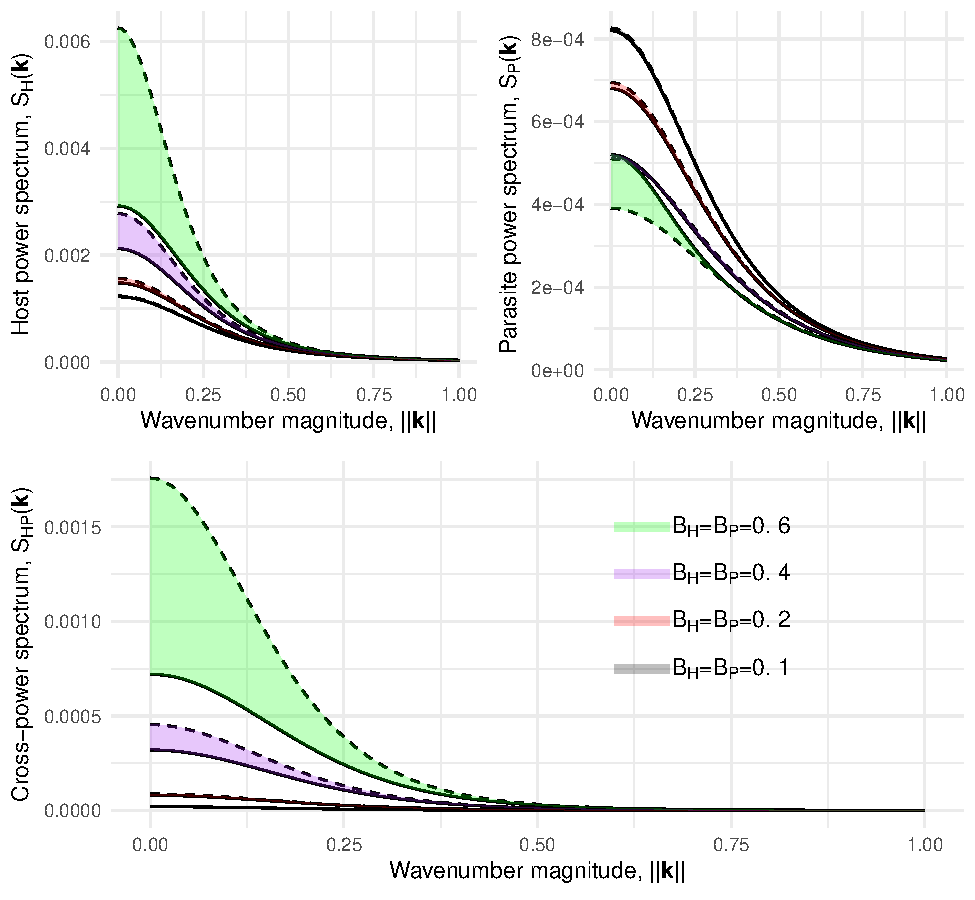
\includegraphics{Spatial-Scales-of-Local-Adaptation-in-Host-Parasite-Coevolution_files/figure-latex/unnamed-chunk-1-1.pdf}
\caption{Comparisons of approximated power spectra (dashed lines) to
exact power spectra (solid lines) for four different strengths of biotic
(coevolutionary) selection \(B=0.1,0.2,0.4,0.6\). For simplicity, biotic
selection on host and parasite are set equal (\(B_H=B_P=B\)). Background
parameters are set to \(A_H=A_P=1\), \(G_H=G_P=10\),
\(\sigma_H=\sigma_P=10\) and \(N_H=N_P=100\). Our model only is defined
for \(B_H<A_H\). Hence, the behaviour of power spectra as \(B\)
increases reflects what happens when the host comes closer to being able
to overcome abiotic stabilizing selection and escape parasitism. In this
limit, we see that our approximations over estimate the magnitudes of
low frequency content in the host spatial covariance and host-parasite
cross-covariance. This implies that our approximations over estimate the
spatial scale of phenotypic covariance of the host and phenotypic
cross-covariance of the host and parasite when coevolution is strong. In
contrast, we see that our approximations under estimate the amount of
low frequency content in the spatial covariance of parasite traits. This
implies that our approximations under estimate the spatial scale of
phenotypic covariance of the parasite when coevolution is strong.
However, when coevolution is relatively weak, say one-tenth the strength
of abiotic selection, we see our approximation matches closely the exact
power spectra.}
\end{figure}

Using common notation for describing covariance structures of random
fields, we denote by \(\xi_S\) the characteristic scale of spatial trait
covariance for species \(S=H,P\) and by \(V_S\) the marginal variance of
the same species. The marginal variance \(V_S\) can be thought of as a
measure of uncertainty when observing local mean traits as well as the
expected sample variance for mean traits sampled far enough apart.
Setting

\[\xi_H=\frac{\sigma_H}{\sqrt{G_HA_H}}, \ \xi_P=\frac{\sigma_P}{\sqrt{G_PA_P}},\]

\[V_H=\frac{1}{N_H\sigma_H^2A_H}, \ V_P=\frac{1}{N_P\sigma_P^2A_P},\]

the approximated power spectra can be rewritten as

\[S_H(\pmb k)\approx \frac{V_H\xi_H^2}{(1+\frac{1}{2}\xi_H^2\|\pmb k\|^2)^2}, \ S_P(\pmb k)\approx \frac{V_P\xi_P^2}{(1+\frac{1}{2}\xi_P^2\|\pmb k\|^2)^2}\]

\[S_{HP}(\pmb k)\approx \frac{B_P}{A_P}\frac{1}{1+\frac{1}{2}\xi_P^2\|\pmb k\|^2}S_H(\pmb k)-\frac{B_H}{A_H}\frac{1}{1+\frac{1}{2}\xi_H^2\|\pmb k\|^2}S_P(\pmb k).\]

The cross-spectrum can be simplified in few special cases. First, in the
case where \(\xi_H=\xi_P=\xi\) we have

\[S_{HP}^{\{\xi_H=\xi_P=\xi\}}(\pmb k)\approx\left(V_H\frac{B_P}{A_P}-V_P\frac{B_H}{A_H}\right)\frac{\xi^2}{\left(1+\tfrac{1}{2}\xi^2\|\pmb k\|^2\right)^3}.\]

Since the cases where \(\xi_P\to0\) and \(\xi_H\to0\) respectively imply
\(\sigma_P\to0\) and \(\sigma_H\to0\) (assuming finite additive genetic
variances and selection strengths), we consider the power spectra in
terms of the biological parameters above. In these two cases we see the
intraspecific power spectra become

\[S_H^{\{\sigma_H\to0\}}(\pmb k)\approx\frac{1}{N_HA_H}, \ S_P^{\{\sigma_P\to0\}}(\pmb k)\approx\frac{1}{N_PA_P}.\]

Then it follows the interspecific cross-spectrum becomes

\[S_{HP}^{\{\sigma_P\to0\}}(\pmb k)\approx\frac{B_P}{A_P}S_H(\pmb k)-\frac{B_H}{N_PA_HA_P},\]

\[S_{HP}^{\{\sigma_H\to0\}}(\pmb k)\approx\frac{B_P}{N_HA_HA_P}-\frac{B_H}{A_H}S_P(\pmb k).\]

The spatial covariance functions, equal to the inverse Fourier
transforms of the power spectra
\(S_H(\pmb k),S_P(\pmb k),S_{HP}(\pmb k)\), can then be approximated as

\[C_H(\pmb x)\approx V_H\sqrt2\frac{\|\pmb x\|}{\xi_H}K_1\left(\sqrt2\frac{\|\pmb x\|}{\xi_H}\right),\]

\[C_P(\pmb x)\approx V_P\sqrt2\frac{\|\pmb x\|}{\xi_P}K_1\left(\sqrt2\frac{\|\pmb x\|}{\xi_P}\right),\]

where \(K_\nu\) is a modified Bessel function of the second kind, order
\(\nu\). Conveniently, the approximated spatial covariance functions
take the form of a Matérn covariance functions, which are widely applied
in the fields of spatial statistics (refs) and machine learning (ref).
In general, the Matérn covariance function takes the form

\[M_\nu(\pmb x|\xi,V)=V\frac{2^{1-\nu}}{\Gamma(\nu)}\left(\sqrt{2\nu}\frac{\|\pmb x\|}{\xi}\right)^\nu K_\nu\left(\sqrt{2\nu}\frac{\|\pmb x\|}{\xi}\right).\]

Hence, \(C_S(\pmb x)=M_1(\pmb x|\xi_S,V_S)\) for both \(S=H,P\). With
this notation, the interspecific spatial cross-covariance function can
be approximated by

\[C_{HP}(\pmb x)\approx 2\int_{\mathbb R^2}\frac{B_P}{A_P}\frac{K_0(\|\pmb y\|/\xi_P)}{\xi_P^2}M_1(\pmb x-\pmb y|\xi_H,V_H)-\frac{B_H}{A_H}\frac{K_0(\|\pmb y\|/\xi_H)}{\xi_H^2}M_1(\pmb x-\pmb y|\xi_P,V_P)d\pmb y.\]

\begin{itemize}
\item
  \(K_0(\|\pmb x\|)\) is positive integrable and square integrable
  function of \(\pmb x\), which suggests the convolution with
  \(M_1(\pmb x|\xi,V)\) produces a legit covariance function.
\item
  Still need to check that this cross-covariance function is copacetic
  with the intraspp cov fcts. how to check?
\end{itemize}

\[\mathcal F\{C_{HP}/\sqrt{C_HC_P}\}=\hat C_{HP}*\mathcal F\{1/\sqrt{C_H}\}*\mathcal F\{1/\sqrt{C_P}\}\]

In general, this cross-covariance function is not Matérn. However, under
the special cases listed above, this cross-covariance function does take
the form of a Matérn function. In particular, under the respective
special cases we get

\[C_{HP}^{\{\xi_H=\xi_P=\xi\}}(\pmb x)\approx\left(V_H\frac{B_P}{A_P}-V_P\frac{B_H}{A_H}\right)2\frac{\|\pmb x\|^2}{\xi^2}K_2\left(2\frac{\|\pmb x\|}{\xi}\right),\]

\[C_{HP}^{\{\xi_P\ll\xi_H\}}(\pmb x)\approx\frac{B_P}{A_P}V_H\sqrt2\frac{\|\pmb x\|}{\xi_H}K_1\left(\sqrt2\frac{\|\pmb x\|}{\xi_H}\right),\]

\[C_{HP}^{\{\xi_H\ll\xi_P\}}(\pmb x)\approx-\frac{B_H}{A_H}V_P\sqrt2\frac{\|\pmb x\|}{\xi_P}K_1\left(\sqrt2\frac{\|\pmb x\|}{\xi_P}\right).\]

In each of these special cases the notions of spatial scale for
cross-covariance, which provides a notion of spatial scale of
coevolution, are trivially defined respectively by \(\xi\), \(\xi_H\)
and \(\xi_P\). Research on the spatial dynamics of host-parasite
coevolution has focused on cases of differential migration patterns and
selection strengths, resulting here in distinct spatial scales of
intraspecific variation. Since our SPDE model predicts Matérn functions
that describe spatial cross-covariation between coevolving species
require equivalent intraspecific spatial scales, we see that they fall
short of capturing the more realistic and interesting biological
scenarios.

The general cross-covariance function above is rather unwieldy, making
its direct study difficult. An alternative quantity to consider is the
so-called \emph{coherence function}, which describes linear
relationships between two random fields at each frequency in their
spectral representations. In particular, interspecific coherence is
defined by

\[\kappa_{HP}(\pmb k)=\frac{S_{HP}(\pmb k)}{\sqrt{S_H(\pmb k)S_P(\pmb k)}}.\]

This function can be used to compute frequencies of maximal coherency,
which provides information about the spatial scale of interspecific
covariance (and thus a notion for the spatial scale of interspecific
coevolution). Before examining the general case, we consider the special
cases where the cross-covariance function is Matérn. In general, for a
pair of random fields having Matérn covariance functions with smoothness
\(\nu_i\) and scale \(\xi_i\) for the \(i\)th field and
\(\nu_{12},\xi_{12}\) for the cross-smoothness and cross-scale, the
frequencies \(\|\pmb k\|^2\) that maximize the square coherency function
\(|\kappa_{12}(\pmb k)|^2\) are known to solve

\[\frac{\nu_1+d/2}{2\nu_1/\xi_1^2+\|\pmb k\|^2}+\frac{\nu_2+d/2}{2\nu_2/\xi_2^2+\|\pmb k\|^2}-\frac{2\nu_{12}+d}{2\nu_{12}/\xi_{12}^2+\|\pmb k\|^2}=0.\]

Following our results above, in the special case of \(\xi_H=\xi_P=\xi\)
we obtain maximum square coherence at frequency
\(\|\pmb k\|=\sqrt2/\xi\). This suggests that the frequency of maximum
square coherence is inversely proportional to the spatial scale of
coevolution. In both cases where one species disperses a much greater
distance than the other and we take the perspective of the greater
disperser (so that the dispersal distance of the shorter disperser is
sent to zero) the square coherence is maximized at
\(\|\pmb k\|=+\infty\) which, by the same reasoning, would suggest the
spatial scale of coevolution is zero. In general, coherence under our
model takes the form

\[\kappa_{HP}(\pmb k)=\sqrt\frac{V_H}{V_P}\frac{B_P}{A_P}\frac{\xi_H/\xi_P}{1+\tfrac{1}{2}\xi_H^2\|\pmb k\|^2}-\sqrt\frac{V_P}{V_H}\frac{B_H}{A_H}\frac{\xi_P/\xi_H}{1+\tfrac{1}{2}\xi_P^2\|\pmb k\|^2}.\]

The square of this coherence function is maximized at

\[\|\pmb k^*\|^2=2\frac{V_PB_HA_P\xi_H^{-2}-V_HB_PA_H\xi_P^{-2}\pm\sqrt{V_HV_PB_HB_PA_HA_P}|\xi_P^{-2}-\xi_H^{-2}|}{V_PB_PA_H-V_HB_HA_P}.\]

It can be verified that the three special cases treated above can be
derived from this general solution. A unique solution exists when

\[\left(\frac{V_HB_PA_H}{V_PB_HA_P}-1\right)\xi_H^4<\left(1-\frac{V_PB_HA_P}{V_HB_PA_H}\right)\xi_P^4.\]

Under these conditions we can define the spatial scale of coevolution as
\(\xi_{HP}=\sqrt2/\|\pmb k^*\|\). When these conditions are not met
either no solution exists or two solutions exist. In the case of two
solutions, denote them by \(\|\pmb k_1^*\|^2\) and \(\|\pmb k_2^*\|\),
we can extend the definition of the spatial scale of coevolution to
\(\xi_{HP}=2/\sqrt{\|\pmb k_1^*\|^2+\|\pmb k_2^*\|^2}\) which returns
the original definition when \(\|\pmb k_1^*\|=\|\pmb k_2^*\|\). Lastly,
we note that when one species disperses much greater than the other and
we take the perspective of the shorter disperser (so that either
\(\sigma_H\to+\infty\) or \(\sigma_P\to+\infty\)), we obtain
\(\|\pmb k^*\|=0\) which implies the spatial scale of coevolution is
infinite in these cases. Since the cross-covariance is zero in these
cases we had no way to define this scale previously. Pairing with our
results above where we considered the scale of the greater disperser, we
see that whether the spatial scale of coevolution is zero or infinity
depends on whether we take the perspective of the longer or shorter
disperser respectively.

\hypertarget{marginal-values-and-integrals-of-spatial-covariance-and-cross-covariance-functions}{%
\subsection{Marginal values and integrals of spatial covariance and
cross-covariance
functions}\label{marginal-values-and-integrals-of-spatial-covariance-and-cross-covariance-functions}}

Following results from section A, the marginal covariance of species
mean traits can be approximated via

\[C_{HP}(\pmb 0)=\frac{1}{2\pi}\int_{\mathbb R^2}S_{HP}(\pmb k)d\pmb k\]

\[\approx \frac{G_HG_P}{\sigma_H^2\sigma_P^2}\frac{\xi_H^2\xi_P^2}{(\xi_H^2-\xi_P^2)^2}\left[\frac{B_P}{N_H\sigma_H^2}\Big(\xi_H^4+\xi_H^2\xi_P^2(\ln\xi_P^2-\ln\xi_H^2-1)\Big)\right.\]

\[\left.-\frac{B_H}{N_P\sigma_P^2}\Big(\xi_P^4+\xi_H^2\xi_P^2(\ln\xi_H^2-\ln\xi_P^2-1)\Big)\right].\]

This marginal covariance turns out to be central to our definition of
local adaptation in continuous space. However, below we consider
alternative definitions of local adaptation and they depend on different
functionals of the spatial cross-covariance function. Hence, we list
here the needed results for our alternative definitions of local
adaptation.

The integral of \(C_{HP}(\pmb x)\) is approximated via

\[\int_{\mathbb R^2}C_{HP}(\pmb x)d\pmb x=2\pi S_{HP}(\pmb 0)\approx2\pi\left(\frac{B_P}{A_P}V_H\xi_H^2-\frac{B_H}{A_H}V_H\xi_H^2\right)\]

\[=2\pi \left(\frac{B_P}{G_HN_HA_H^2A_P}-\frac{B_H}{G_PN_PA_HA_P^2}\right).\]

Note that the integral \(\int_{\mathbb R^2}C_{HP}(\pmb x)d\pmb x\) is
biased by larger distances. To see this we can change our integration to
polar coordinates to find
\(\int_{\mathbb R^2}C_{HP}(\pmb x)d\pmb x=2\pi\int_0^\infty C_{HP}(r)rdr\).
To remove this bias we calculate \(\int_0^\infty C_{HP}(r)dr\).
Switching this integral back to Cartesian coordinates yields

\[\int_0^\infty C_{HP}(r)dr=\frac{1}{2\pi}\int_{\mathbb R^2}\frac{1}{\|\pmb x\|}C_{HP}(\pmb x)d\pmb x.\]

To evaluate \(\int_0^\infty C_{HP}(r)dr\), we can use the relationship

\[\int_{\mathbb R^2}\frac{1}{\|\pmb x\|}C_{HP}(\pmb x)d\pmb x=\mathcal F\left\{\frac{C_{HP}(\pmb x)}{\|\pmb x\|}\right\}_{\pmb k=\pmb 0},\]

where \(\mathcal F\) denotes Fourier transformation and the subscript
denotes evaluation at \(\pmb k=\pmb 0=(0,0)^\top\). Taking the Fourier
transform of \(C_{HP}(\pmb x)/\|\pmb x\|\), we find

\[\mathcal F\left\{\frac{C_{HP}(\pmb x)}{\|\pmb x\|}\right\}\approx\frac{B_P}{A_P}\frac{1}{1+\frac{1}{2}\xi_P^2\|\pmb k\|^2} \frac{V_H\xi_H/\sqrt2}{1+\frac{1}{2}\xi_H^2\|\pmb k\|^2}E\left(-\frac{1}{2}\xi_H^2\|\pmb k\|^2\right)\]

\[-\frac{B_H}{A_H}\frac{1}{1+\frac{1}{2}\xi_H^2\|\pmb k\|^2} \frac{V_P\xi_P/\sqrt2}{1+\frac{1}{2}\xi_P^2\|\pmb k\|^2}E\left(-\frac{1}{2}\xi_P^2\|\pmb k\|^2\right),\]

where \(E(\zeta)=\int_0^{\pi/2}\sqrt{1-\zeta\sin^2\theta}d\theta\) is an
elliptic integral. In particular, this provides

\[\mathcal F\left\{\frac{C_{HP}(\pmb x)}{\|\pmb x\|}\right\}_{\pmb k=\pmb 0}\approx\frac{\pi}{2}\left(\frac{B_P}{A_P}\frac{\xi_H}{\sqrt2}V_H-\frac{B_H}{A_H}\frac{\xi_P}{\sqrt2}V_P\right).\]

We therefore conclude

\[\int_0^\infty C_{HP}(r)dr\approx\frac{1}{4\sqrt2}\left(\frac{B_P}{A_P}\xi_HV_H-\frac{B_H}{A_H}\xi_PV_P\right)\]

\[=\frac{1}{4\sqrt2}\left(\frac{B_P}{A_P}\frac{\xi_H}{\sqrt2}V_H-\frac{B_H}{A_H}\left(A_P^{3/2}N_P\sigma_P\sqrt{G_P}\right)^{-1}\right).\]

Using the same trick to compute the integral lengths of intraspecific
phenotypic variation, we find

\[\int_0^\infty C_S(r)dr=\frac{1}{2\pi}\lim_{\pmb k\to\pmb 0}\mathcal F\left\{\frac{C_S(\pmb x)}{\|\pmb x\|}\right\}\approx\frac{V_S\xi_S}{4\sqrt2}.\]

The quantity \(\mathcal I_S=\int_0^\infty C_S(r)dr\) has been referred
to as the integral length of spatial covariance (here the integral
length of intraspecific spatial covariance). Then, an integral length of
interspecific spatial covariance may be computed as

\[\mathcal I_{HP}:=\int_0^\infty |C_{HP}(r)|dr.\]

Assuming \(C_{HP}(r)\) is either always positive or always negative
allows us to move the absolute value outside of the integral. Then,
under our model, we find

\[\mathcal I_{HP}\approx\frac{1}{4\sqrt2}\left|\frac{B_P}{A_P}V_H\xi_H-\frac{B_H}{A_H}V_P\xi_P\right|\]

\[=\frac{1}{4\sqrt2}\left|\frac{B_P}{A_PA_H^{3/2}}\frac{1}{\sigma_H N_H\sqrt{G_H}}-\frac{B_H}{A_HA_P^{3/2}}\frac{1}{\sigma_P N_P\sqrt{G_P}}\right|.\]

\hypertarget{measures-of-local-adaptation}{%
\section{\texorpdfstring{Measures of local adaptation
\label{la-app}}{Measures of local adaptation }}\label{measures-of-local-adaptation}}

\begin{itemize}
\tightlist
\item
  use \(\mathcal L\) for measures in terms of mean fitness and \(\ell\)
  for measures in terms of log-mean fitness
\end{itemize}

Local adaptation is commonly measured as the difference in fitness for
individuals experiencing their local environment and fitness for
individuals experiencing foreign environments (Gandon \& Nuismer 2009,
Nuismer 2017, etc). In the case of coevolution, the environmental
variable is replaced by the trait value of the interacting partner
species.

yada yada yada, folks end up with something like
\(\mathcal L_P=\tilde\alpha-\tilde\alpha_0\). Using a slightly different
definition, parasite local adaptation simplifies to
\(\ell_P=\widetilde{\ln\alpha}-\widetilde{\ln\alpha}_0=B_PC_{HP}(0)\).

Here extend this notion of local adaptation to the case of populations
distributed continuously in space. In particular, we denote by
\(\Delta_H(\pmb y)\) the difference in expected population growth rates
of the host when confronted with parasites drawn from a spatial lag
\(\pmb y=(y_1,y_2)^\top\) away. That is,

\[\Delta_H(\pmb y)=\mathbb E[m_H(\bar z_H(\pmb x),\bar z_P(\pmb x))-m_H(\bar z_H(\pmb x),\bar z_P(\pmb x+\pmb y))].\]

We define \(\Delta_P(\pmb y)\) in a complementary manner for the
parasite species. Under our model of trait matching/mis-matching,
\(\Delta_H(\pmb y)\) simplifies to

\[\Delta_H(\pmb y)=\mathbb E\left[\frac{B_H}{2}\left(\bar z_H(\pmb x)-\bar z_P(\pmb x)\right)^2-\frac{B_H}{2}\left(\bar z_H(\pmb x)-\bar z_P(\pmb x+\pmb y)\right)^2\right]=B_H\left(C_{HP}(\|\pmb y\|)-C_{HP}(0)\right),\]

where \(\|\pmb y\|=\sqrt{y_1^2+y_2^2}\). Similarly, we obtain
\(\Delta_P(\pmb y)=B_P(C_{HP}(0)-C_{HP}(\|\pmb y\|))\) for the parasite.
Now, if we consider picking \(\pmb y\) at random from a disc of radius
\(h\) centered on the origin (ie, \(U_h=\{\pmb x:\|\pmb x\|<h\}\)), the
probability that \(h/2<\|\pmb y\|<h\) is \(3/4\). Hence, there is a
greater probability that \(\|\pmb y\|\) will be closer to \(h\) than to
zero. Then, considering uniform random sampling of the plane
\(\mathbb R^2\) as the limit of sampling from \(U_h\) as \(h\to\infty\),
we can expect any \(\pmb y\) randomly sampled from the plane to have
infinite length. This sampling process is analogous to the global random
sampling process used in definitions of local adaptation for
metapopulation models. Then, to define a comparable measure of local
adaptation for continuously distributed populations we set

\[\ell_S^\infty:=\lim_{\|\pmb y\|\to\infty}\Delta_S(\pmb y).\]

There are alternative notions of local adaptation we can consider that
provide different perspectives. For example, we could consider
integrating \(\Delta_S(\pmb y)\) across the entire plane to obtain a
different global measure of local adaptation. The idea here is to
account for fitness differences measured at all possible distances
instead of a random distance. We define this measure as
\(\invbreve{\ell}_S:=\int_{\mathbb R^2}\Delta_S(\pmb y)d\pmb y\). Using
our results from section A, we obtain

\[\invbreve{\ell}_H\approx B_H\left(\frac{B_H}{G_PN_PA_HA_P^2}-\frac{B_P}{G_HN_HA_H^2A_P}\right),\]

\[\invbreve{\ell}_P\approx B_P\left(\frac{B_P}{G_HN_HA_H^2A_P}-\frac{B_H}{G_PN_PA_HA_P^2}\right).\]

This measure of local adaptation depends on the effective densities
\(N_H,N_P\) which suggests it provides some indication for the role of
random genetic drift in determining global patterns of local adaptation.
However, it does not dependent on dispersal distances because of the
extra weight given to larger distances implicit in this definition.
Hence, it provides no information on the role of gene-flow in
determining global patterns of local adaptation. To circumvent this
issue, we define another index that explicitly integrates across
distances. In particular, we define
\(\tilde{\ell}_S=\int_0^\infty\tilde\Delta_S(h\pmb e)dh\) where
\(\pmb e=(1/\sqrt2,1/\sqrt2)^\top\). Using our results from above, we
find

\[\tilde{\ell}_H\approx\frac{B_H}{4}\left(\frac{B_H}{A_H}\frac{\xi_P}{\sqrt2}-\frac{B_P}{A_P}\frac{\xi_H}{\sqrt2}\right),\]

\[\tilde{\ell}_P\approx\frac{B_P}{4}\left(\frac{B_P}{A_P}\frac{\xi_H}{\sqrt2}-\frac{B_H}{A_H}\frac{\xi_P}{\sqrt2}\right).\]

Since \(\xi_S\propto\sigma_S\) for \(S=H,P\) we see that this
alternative global index of local adaptation captures the role of
gene-flow. However, the absence effective densities in these expressions
suggests \(\tilde{\ell}_H,\tilde{\ell}_P\) do not capture the effects of
random genetic drift. Hence, the two sets of indices
\((\invbreve{\ell}_H,{\ell}_P)\) and \((\tilde{\ell}_H,\tilde{\ell}_P)\)
capture complementary aspects of global patterns of local adaptation
driven by interactions between gene-flow, drift, abiotic stabilizing
selection, and host-parasite coevolution.

\hypertarget{a-local-measure-of-local-adaptation}{%
\subsection{A local measure of local
adaptation}\label{a-local-measure-of-local-adaptation}}

The global measure of local adaptation defined above considered the
difference in fitness at two points in space drawn uniformly at random.
Hence, the global measure captures the idea of comparing host fitness
when confronted with a local parasite to host fitness when confronted to
a parasite drawn at random from any location. Since the expected
distance between random locations drawn from an infinite plane is
infinite, this global measure ignores the effects of spatial
autocorrelation. However, the range sizes of empirical host-parasite
systems may not be large enough to ignore spatial autocorrelation.
Hence, a local measure of local adaptation is needed.

Writing \(D_S(\pmb y)\) as the dispersal kernel for species \(S\), we
can compute the average spatial fitness difference with respect to this
dispersal kernel as
\(\bar\Delta_S:=\int_{\mathbb R^2}\Delta_S(\pmb y)D_S(\pmb y)d\pmb y\).
To compute this average we use the relation
\(\int_{\mathbb R^2}\Delta_S(\pmb y)D_S(\pmb y)d\pmb y=\int_{\mathbb R^2}\hat\Delta_S(\pmb k)\hat D_S(\pmb k)d\pmb k\),
where \(\hat\Delta_S(\pmb k)\) and \(\hat D_S(\pmb k)\) are respectively
the Fourier transforms of \(\Delta_S(\pmb x)\) and \(D_S(\pmb x)\).

We denote by \(D(\pmb x)\) the probability density that two individuals
of opposing species were separated by \(\pmb x\) before dispersal given
that they end up at the same location after dispersal. We refer to
\(D(\pmb x)\) as the separation kernel. Since we assume dispersal for
each species is bivariate Gaussian with respective standard deviations
(in both coordinates) \(\sigma_H,\sigma_P\), \(D(\pmb x)\) will also be
bivariate Gaussian with standard deviation
\(\sqrt{\sigma_H^2+\sigma_P^2}\).

Whereas local adaptation is classically measured as the difference
between fitness ``at home'' versus fitness in a randomly selected
environment, the limited dispersal analog is fitness ``at home'' versus
fitness in a randomly selected environment weighted by the separation
kernel. In particular, for species \(S=H,P\),

\[\invbreve{\mathcal L}_S=\mathbb E[\bar w_S(\pmb x,\pmb x)]-\mathbb E\left[\int_{\mathbb R^2}\bar w_S(\pmb x,\pmb x+\pmb y)D(\pmb y)d\pmb y\right],\]

where \(\bar w_H(\pmb x,\pmb y)\) and \(\bar w_P(\pmb x,\pmb y)\) are
shorthand for \(\bar w_H(\bar z_H(\pmb x),\bar z_P(\pmb y)\) and
\(\bar w_P(\bar z_P(\pmb x),\bar z_H(\pmb y))\) respectively. Applying
the trait matching/mis-matching model of fitness, we obtain

\[\invbreve{\mathcal L}_H=\cdots\]

\[\invbreve{\mathcal L}_P=\cdots\]

For the sake of clarity, we focus on a closely related measure of local
adaptation that utilizes the local population growth rate \(\bar m_S\)
instead of the population mean fitness \(\bar w_S\) for species
\(S=H,P\). In particular, we define

\[\invbreve\ell_S=\mathbb E[\bar m_S(\pmb x,\pmb x)]-\mathbb E\left[\int_{\mathbb R^2}\bar m_S(\pmb x,\pmb x+\pmb y)D(\pmb y)d\pmb y\right],\]

where \(\bar m_H(\pmb x,\pmb y)\) and \(\bar m_P(\pmb x,\pmb y)\) are
shortand for \(\bar m_H(\bar z_H(\pmb x),\bar z_P(\pmb y)\) and
\(\bar m_P(\bar z_P(\pmb x),\bar z_H(\pmb y))\) respectively. Applying
the trait matching/mis-matching model of fitness along with our
assumption of spatially homogeneous abiotic stabilizing selection, we
obtain

\begin{multline}
  \mathbb E[\bar m_H(\pmb x,\pmb x)]=
  r_H-\frac{A_H}{2}[(\theta_H-\mu_H)^2+v_H+V_H]
  +\frac{B_H}{2}[(\mu_H-\mu_P)^2+v_H+v_P+V_H+V_P] \\
  -B_HC_{HP}(0),
\end{multline}

\begin{multline}
  \mathbb E\left[\int_{\mathbb R^2}\bar m_H(\pmb x,\pmb y)
  D(\pmb y)d\pmb y\right]= 
  r_H-\frac{A_H}{2}[(\theta_H-\mu_H)^2+v_H+V_H] \\
  +\frac{B_H}{2}[(\mu_H-\mu_P)^2+v_H+v_P+V_H+V_P]
  -B_H\int_{\mathbb R^2}C_{HP}(\pmb y)D(\pmb y)d\pmb y,
\end{multline}

\begin{multline}
  \mathbb E[\bar m_P(\pmb x,\pmb x)]=
  r_P-\frac{A_P}{2}[(\theta_P-\mu_P)^2+v_P+V_P]
  -\frac{B_P}{2}[(\mu_P-\mu_H)^2+v_P+v_H+V_P+V_H] \\
  +B_P C_{HP}(0),
\end{multline}

\begin{multline}
  \mathbb E\left[\int_{\mathbb R^2}\bar m_P(\pmb x,\pmb y)
  D(\pmb y)d\pmb y\right]= 
  r_P-\frac{A_P}{2}[(\theta_P-\mu_P)^2+v_P+V_P] \\
  -\frac{B_P}{2}[(\mu_P-\mu_H)^2+v_P+v_H+V_P+V_H]
  +B_P\int_{\mathbb R^2}C_{HP}(\pmb y)D(\pmb y)d\pmb y,
\end{multline}

Setting \(\bar C_{HP}\int_{\mathbb R^2}C_{HP}(\pmb y)D(\pmb y)d\pmb y\),
the expressions for local adaptation accounting for limited dispersal
simplify to

\[\invbreve{\ell}_H=B_H\left(\bar C_{HP}-C_{HP}(0)\right),\]

\[\invbreve{\ell}_P=B_P\left(C_{HP}(0)-\bar C_{HP}\right).\]

\hypertarget{scotts-measure-of-coevolutionary-advantage}{%
\subsection{Scott's measure of coevolutionary
advantage}\label{scotts-measure-of-coevolutionary-advantage}}

\[\mathcal a=\bar{\bar m}-\bar{\bar m}^0\]

where \(\bar{\bar m}^0\) is the spatial average of growth rate in the
absence of biotic selection. Setting \(\bar{\bar z}_S^0, V_S^0\) the
spatial mean and variance of local mean traits for species \(S\) and
\(C_{HP}^{S,0}\) the covariance of mean traits between species when
\(B_S=0\), our model assumptions then implies

\begin{multline}
  \mathcal a_P=B_P(C_{HP}-C_{HP}^{P,0})-\frac{B_P}{2}\big[(\bar{\bar z}_H-\bar{\bar z}_P)^2+V_H+V_P+v_H+v_P\big] \\
  -\frac{A_P}{2}\big[(\theta_P-\bar{\bar z}_P)^2-(\theta_P-\bar{\bar z}_P^0)^2+V_P-V_P^0\big],
\end{multline}

\begin{multline}
  \mathcal a_H=-B_P(C_{HP}-C_{HP}^{H,0})+\frac{B_H}{2}\big[(\bar{\bar z}_P-\bar{\bar z}_H)^2+V_H+V_P+v_H+v_P\big] \\
  -\frac{A_H}{2}\big[(\theta_H-\bar{\bar z}_H)^2-(\theta_H-\bar{\bar z}_H^0)^2+V_H-V_H^0\big].
\end{multline}

\begin{itemize}
\tightlist
\item
  NOTE: Scott defines this measure by comparing the coevolutionary
  scenario to the no biotic selection for both species scenario. In this
  case it seems possible that \(\mathcal a\) can be positive for both
  species, blurring the distinction of which species is ``winning'' the
  coevolutionary race. Alternatively, we can proceed as above and
  consider the case when just one or the other species incurs zero
  biotic selection.
\end{itemize}

\hypertarget{the-discrete-geography-models}{%
\subsection{The discrete geography
models}\label{the-discrete-geography-models}}

\hypertarget{global-dispersal}{%
\subsubsection{Global dispersal}\label{global-dispersal}}

To study the role of geography, we consider and extreme alternative to
our continuous space model. In particular, we assume dispersal is global
and follows a metapopulation model with \(n\) locations. Individuals
move between locations at a fixed rate for each species. We denote these
migration rates by \(\omega_H,\omega_P\geq0\). Then, denoting
\(\mu_S(t)\) the average of \(\bar z_S(t)\) across locations, our
discrete geography model is

\[\dot{\bar z}_H=G_HA_H(\theta_H-\bar z_H)-G_HB_H(\bar z_P-\bar z_H)+\omega_H(\mu_H-\bar z_H)+\sqrt\frac{G_H}{N_H}\dot W_H,\]

\[\dot{\bar z}_P=G_PA_P(\theta_P-\bar z_P)+G_PB_P(\bar z_H-\bar z_P)+\omega_P(\mu_P-\bar z_P)+\sqrt\frac{G_P}{N_P}\dot W_P.\]

Here \(N_S\) is no longer a spatial density of abundance, but the
measure of abundance at any location in this discrete geography. Since
our goal is to compute
\(C_{HP}=\tfrac{1}{n}\sum_{i=1}^n(\bar z_H(i)-\mu_H)(\bar z_P(i)-\mu_P)\)
at equilibrium we can set \(\theta_H=\theta_P=\mu_H=\mu_P=0\) without
loss of generality. In addition, using our assumption that
\(A_S\gg B_S\) the discrete space model simplifies to

\[\dot{\bar z}_H=-(G_HA_H+\omega_H)\bar z_H-G_HB_H\bar z_P+\sqrt\frac{G_H}{N_H}\dot W_H,\]

\[\dot{\bar z}_P=-(G_PA_P+\omega_P)\bar z_P+G_PB_P\bar z_H+\sqrt\frac{G_P}{N_P}\dot W_P.\]

We use the Ito product rule to get

\[\dot C_{HP}=\tfrac{1}{n}\sum_{i=1}^n\bar z_H\dot{\bar z}_P+\bar z_P\dot{\bar z}_H.\]

Expanding and taking the limit \(n\to\infty\) provides

\[\dot C_{HP}=-(G_PA_P+\omega_P)C_{HP}+G_PB_PV_H-(G_HA_H+\omega_H)C_{HP}-G_HB_HV_P,\]

where \(V_S=\lim_{n\to\infty}\tfrac{1}{n}\sum_{i=1}^n\bar z_S^2(i)\). At
equilibrium we have

\[C_{HP}=\frac{B_{P} G_{P} V_{H}-B_{H} G_{H} V_{P}}{A_{H} G_{H} + A_{P} G_{P} + \omega_{H} + \omega_{P}}.\]

Assuming \(V_H,V_P\) remain fixed while adjusting \(\omega_H,\omega_P\),
the only effect of dispersal is to decrease the magnitude of \(C_{HP}\).
However, to get the full story we need expressions for \(V_H,V_P\) at
equilibrium. Using the same trick as for \(\dot C_{HP}\) we get

\[\dot V_H=-2(G_HA_H+\omega_H)V_H-2G_HB_HC_{HP}+\tfrac{G_H}{N_H},\]

\[\dot V_P=-2(G_PA_P+\omega_H)V_P+2G_PB_PC_{HP}+\tfrac{G_P}{N_P}.\]

With this information we can compute the interspecific spatial
correlation of local mean trait values at equilibrium. Assuming
parameters are equal except for dispersal rates, the numerator of the
interspecific spatial correlation coefficient is proportional to
\(\omega_{P} - \omega_{H}\). The denominator of the correlation is
always positive under the same symmetry assumptions, so the identity of
the locally adapted species is completely determined by the signage of
the above expression. In particular, this tells use the species that
disperses at a faster rate is locally adapted, all else being equal.

\hypertarget{local-dispersal}{%
\subsubsection{Local dispersal}\label{local-dispersal}}

Here we consider the consequences of local dispersal on local adaptation
in a discrete space stepping model. In particular we assume spatial
localities are arranged on an infinite two-dimensional lattice with
locations identified by \((i,j)\) where \(i,j\in\mathbb Z\). Movement
occurs only between adjacent locations for each species. That is, for a
given location \((i,j)\), the only possible origins of incoming migrants
are \((i+1,j),(i-1,j),(i,j+1),(i,j-1)\). Conversely, these locations are
the only possible destinations for individuals emigrating from
\((i,j)\). Just as in the island model of global dispersal, we denote by
\(\omega_H,\omega_P\) the migration rates for host and parasite
respectively. To obtain the instantaneous rate of change in a mean trait
\(\bar z(i,j)\) due to this form of dispersal, first consider the
discrete time case over an interval of time \(\Delta t\). Denoting
\(\bar z'(i,j)\) the mean trait after dispersal has occurred over the
interval \(\Delta t\) and assuming \(\Delta t\ll1\), we have

\[\bar z'(i,j)=\frac{(1-\omega\Delta t)\bar z(i,j)+4\omega\Delta t\mu(i,j)}{(1-\omega\Delta t)+4\omega\Delta t}\]

where
\(\mu(i,j)=(\bar z(i+1,j)+\bar z(i-1,j)+\bar z(i,j+1)+\bar z(i,j-1))/4\).
Dropping the \((i,j)\), we have

\[\frac{\bar z'-\bar z}{\Delta t}=\frac{4\omega(\mu-\bar z)}{1+3\omega\Delta t},\]

which yields the instantaneous contribution of local dispersal:
\(d\bar z/dt=4\omega(\mu-\bar z)\). Inheriting all other aspects of the
island model above (including intent), we can describe the evolution of
mean traits by the stochastic differential equations

\[\dot{\bar z}_H=-G_HA_H\bar z_H-G_HB_H\bar z_P-4\omega_H(\mu_H-\bar z_H)+\sqrt{\tfrac{G_H}{N_H}}\dot W_H,\]

\[\dot{\bar z}_P=-G_PA_P\bar z_P+G_PB_P\bar z_H+4\omega_P(\mu_P-\bar z_P)+\sqrt{\tfrac{G_P}{N_P}}\dot W_P.\]

Just as for the island model, since our concern is with spatial
covariance we set \(\theta_H=\theta_P=0\). Since this implies
\(\mathbb E[\mu_S(i,j)]=0\) for all \(i,j\in\mathbb Z\) at equilibrium,
we set \(\mu_H=\mu_P=0\) without losing any generality in our
conclusions on \(C_{HP}\). Setting

\[C_{HP}=\lim_{n\to\infty}\frac{1}{4n^2}\sum_{i,j=-n,n}\bar z_H(i,j)\bar z_P(i,j)\]

and for brevity writing \(C_{HP}=\overline{\bar z_H\bar z_P}\), we have

\[\dot C_{HP}=\overline{\bar z_H\dot{\bar z}_P+\dot{\bar z}_H\bar z_P}\]

\[=-G_PA_P\overline{\bar z_H\bar z_P}+G_PB_P\overline{\bar z_H^2}-4\omega_P\overline{\bar z_H\bar z_P}-G_HA_H\overline{\bar z_H\bar z_P}-G_HB_H\overline{\bar z_P^2}-4\omega_H\overline{\bar z_H\bar z_P}\]

\[=-(G_HA_H+G_PA_P+4(\omega_H+\omega_P))C_{HP}+G_PB_PV_H-G_HB_HV_P,\]

where
\(V_S=\overline{\bar z_S^2}=\lim_{n\to\infty}\sum_{i,j=-n,n}\bar z_S^2(i,j)/4n^2\).
Dynamical equations for \(V_H,V_P\) are given by

\[\dot V_H=2\overline{\bar z_H\dot{\bar z}_H}+\tfrac{G_H}{N_H}=-2(G_HA_H+4\omega_H)V_H-2G_HB_HC_{HP}+\tfrac{G_H}{N_H},\]

\[\dot V_P=-2(G_PA_P+4\omega_P)V_P+2G_PB_PC_{HP}+\tfrac{G_P}{N_P}.\]

Since the dynamical equations for \(V_H,V_P,C_{HP}\) under the stepping
stone model match those of the island model, except with dispersal
appearing four times as fast for each species, we obtain the same
qualitative conclusions on the role of relative dispersal abilities in
determining the identity of the locally adapted species.

\hypertarget{justification-for-continuous-space-model}{%
\section{\texorpdfstring{Justification for continuous space model
\label{just}}{Justification for continuous space model }}\label{justification-for-continuous-space-model}}

For the sake of space, we omit any attempt to formally derive our
continuous space model from biological first principles. Instead we
describe a possible approach that can be taken. The level at which we
write is for both the mathematically curious and for the trained
probabilist seeking an outline of ideas employed. We make no claim of
rigor and no promise of general heuristics that can be employed.
Instead, we only provide a schema.

To begin, one may start with a pair of interacting individual-based
branching processes where individuals are associated with a trait
\(z\in\mathbb R\) and a location \(\pmb x\in\mathbb R^2\). Assuming
semelparous life-cycles, we model mortality and reproduction
simultaneously so that individuals replace themselves with a Poisson
number of offspring between exponentially distributed intervals. For
simplicity, we assume the rate at which these branching events occur is
constant. However, the number of offspring is determined by the trait of
the parent along with the traits of other individuals the parent
interacts with. This is similar to the starting points taken by Week et.
al.~(2021a) in the derivation of a diffuse-coevolution model and by Week
et. al.~(2021b) in the derivation of the offset-matching coevolution
model, except neither of those models have a spatial component.

To model fitness, we first consider the effects of abiotic selection
\(\mathcal A_S\) and biotic selection \(\mathcal B_S\) separately for
host and parasite species (\(S=H,P\)). Furthermore, we decompose the
effects of biotic selection into sources due to intraspecific
competition \(\mathcal B_S^c\) and interspecific parasitism
\(\mathcal B_S^p\) so that
\(\mathcal B_S=\mathcal B_S^c\mathcal B_S^p\). We will assume these
effects multiply to produce the net fitness of an individual,
\(w_S=\mathcal A_S\mathcal B_S\). For either species, the multiplicative
component of fitness due to abiotic stabilizing selection for an
individual with trait \(z\) at any location is

\[\mathcal A_S(z)\propto\exp\left(-\frac{A_S}{2}(\theta_S-z)^2\right).\]

We assume competition occurs locally such that individuals that are
geographically closer to each other induce stronger competition on
another than individuals that are further apart. This induces a form of
local population regulation that prevents run-away population growth. In
particular, denoting the distance between two spatial positions
\(\pmb x\) and \(\pmb y\) by \(\|\pmb x-\pmb y\|\), \(\pmb x_i^S\) the
location of the \(i\)th individual in species \(S\), and \(n_S\) the
number of individuals in species \(S\), we model the effect of
intraspecific competition on the \(j\)th individual as

\[\mathcal B_S^c(\pmb x_j,\mathcal N_S)\propto\exp\left(-c_S\sum_{i\neq j}^{n_S}\exp\left(-\frac{\lambda_S}{2}\|\pmb x_j^S-\pmb x_i^S\|^2\right)\right),\]

where \(c_S\) denotes the strength of spatial competition, \(\lambda_S\)
is the rate at which competition decays with distance, and
\(\mathcal N_S\) denotes the abundance measure for species \(S\). In
particular, since \(\mathcal N_S(U,V)\) returns the number of
individuals in species \(S\) with trait values in \(U\subset\mathbb R\)
spatially located in the region \(V\subset\mathbb R^2\),
\(\mathcal N_S\) determines the total abundance and spatial locations of
individuals in species \(S\).

Host-parasite interactions can be modeled by assuming a probability of
infection that is a function of trait values given an encounter has
occurred. In particular, assuming a host individual with trait \(z^H\)
encounters a parasite with trait \(z^P\), the probability of infection
\(\alpha(z^H,z^P)\) can be written as

\[\alpha(z^H,z^P)=\exp\left(-\frac{\gamma}{2}(z^H-z^P)^2\right),\]

where \(\gamma\geq0\) determines the sensitivity of this probability to
differences in individual trait values. We will always assume weak
sensitivity (ie, \(\gamma\ll1\)) so that
\(\alpha(z^H,z^P)\approx1-\gamma(z^H-z^P)^2/2\). We model the
probability of encounter \(\varepsilon\) similarly as a function of the
geographical distance between individuals. Denoting \(\iota\geq0\) the
sensitivity of \(\varepsilon\) to distance and \(\pmb x^S\) the location
of the individual in species \(S\), we model the probability of
encounter as

\[\varepsilon(\pmb x^H,\pmb x^P)=\exp\left(-\frac{\iota}{2}\|\pmb x^H-\pmb x^P\|^2\right).\]

Unlike the sensitivity of the infection probability, we do not assume
\(\iota\ll1\) so that encounters may strongly depend on distance. Then,
assuming the parasite acquires the benefit \(s_P\geq0\) and the host
receives the cost \(s_H\geq0\), the multiplicative effects of this
single interaction on the fitness' of the respective participants are
proportional to
\(\exp(s_P\alpha(z^H,z^P)\varepsilon(\pmb x^H,\pmb x^P))\) and
\(\exp(-s_H\alpha(z^H,z^P)\varepsilon(\pmb x^P,\pmb x^P))\). Then,
assuming every parasite could potentially infect every host, the
components of biotic selection due to interspecific interactions for
each species can be written

\[\mathcal B_H^p(z^H_j,\pmb x^H_j,\mathcal N_P)\propto\exp\left(-s_H\sum_{i=1}^{n_P}\alpha(z^H_j,z^P_i)\varepsilon(\pmb x_j^H,\pmb x_i^P)\right),\]

\[\mathcal B_P^p(z^P_j,\pmb x^P_j,\mathcal N_H)\propto\exp\left(s_P\sum_{i=1}^{n_H}\alpha(z^H_i,z^P_j)\varepsilon(\pmb x_i^H,\pmb x_j^P)\right).\]

To model mutation and spatial movement, we assume offspring trait values
are normally distributed around their parental value (technically, this
is done with breeding values, see Week et. al.~(2021a)) and offspring
locations are bivariate normal around their parental locations with no
correlations between the displacements in the two spatial dimensions
(ie, dispersal is isotropic).

To take a diffusion limit of this individual-base process, we follow
Week et. al.~(2021a) so that the rate of branching goes to infinity, the
number of initial individuals in each species goes to infinity, the
effects of mutation and distances of dispersal go to zero and fitness
for each individual goes to unity. We also rescale the probability of
parasite encounter so that it converges to a delta function. This means
parasitism can only occur locally in the diffusion limit. All of these
limits occur simultaneously and at specific rates to ensure the rescaled
individual-based processes \(\mathcal N_H^{(k)},\mathcal N_P^{(k)}\)
converge to well-defined population-level processes
\(\mathscr N^H,\mathscr N^P\), where \(\mathcal N_S^{(k)}\) denotes the
\(k\)th stage of rescaling. In this diffusion limit the growth rates
associated with trait value \(z\) at location \(\pmb x\) can be obtained
for each species as

\[m_H(z,\pmb x,\mathscr N^H,\mathscr N^P)=\lim_{k\to\infty}k\left(w^{1/k}_H(z,\pmb x,\mathcal N_H^{(k)},\mathcal N_P^{(k)})-1\right),\]

\[m_P(z,\pmb x,\mathscr N^P,\mathscr N^H)=\lim_{k\to\infty}k\left(w^{1/k}_P(z,\pmb x,\mathcal N_P^{(k)},\mathcal N_H^{(k)})-1\right).\]

For the host this yields

\[m_H(z,\pmb x,\mathscr N_H,\mathscr N_P)=r_H-\frac{A_H}{2}(\theta_H-z)^2-c_H\int_{\mathbb R^2}K_H(\pmb x,\pmb y)\mathscr N_H(\mathbb R,d\pmb y)-s_H\int_{\mathbb R^2}\int_{\mathbb R}\alpha(z,\zeta)\mathscr N_P(d\zeta,d\pmb x),\]

where \(r_H\) is some real number (the intrinsic growth rate) and we set
\(K_S(\pmb x,\pmb y)=\exp\left(-\frac{\lambda_S}{2}\|\pmb x-\pmb y\|^2\right)\).
A similar expression for the parasite is also obtained. We now make the
approximation that competition is sufficiently weak and the intrinsic
growth rate is sufficiently positive so that local density of abundance
is approximately constant in time and space for each species. This
implies the population growth rates \(m_H,m_P\) are near zero. With this
approximation we write \(N_S\) as the abundance density for species
\(S\) so that \(\mathscr N_S(\mathbb R,U)=|U|N_S\) for
\(U\subset\mathbb R^2\) where \(|U|\) is the area of \(U\). In this case
we have

\[\int_{\mathbb R^2}K_S(\pmb x,\pmb y)\mathscr N^S(\mathbb R,d\pmb y)=N_S\frac{2\pi}{\lambda_S}.\]

Using our assumption that \(\gamma\ll1\), the biotic and abiotic
components cumulatively contribute quadratic selection. Hence, given
that stabilizing abiotic selection is sufficiently strong relative to
disruptive biotic selection on the host, trait distributions at any
location will be approximately normal with mean and variance
\(\bar z_S(\pmb x),v_S(\pmb x)\) for species \(S\) at location
\(\pmb x\). In particular, this implies

\[\int_{\mathbb R^2}\int_{\mathbb R}\alpha(z,\zeta)\mathscr N^P(d\zeta,d\pmb x)=N_S\left(1-\frac{\gamma}{2}(z-\bar z_P(\pmb x))^2+v_P(\pmb x)\right).\]

Furthermore, since selection is quadratic and abundance is constant,
selection and drift decay phenotypic variance at a constant rate. From
our assumption of Gaussian mutations, phenotypic variance also has a
constant rate of input. Hence, we can expect phenotypic variance for
each species to fluctuate stochastically around an equilibrium that is
constant in space and time. We thus further approximate by setting the
phenotypic variances equal to those constant equilibria. We can
therefore approximate the growth rates for each species as

\[m_H(z,\pmb x)\approx R_H-\frac{A_H}{2}(\theta_H-z)^2+\frac{B_H}{2}(z-\bar z_P)^2,\]

\[m_P(z,\pmb x)\approx R_P-\frac{A_P}{2}(\theta_P-z)^2-\frac{B_P}{2}(z-\bar z_P)^2,\]

where \(R_H,R_P>0\), \(B_P=s_PN_H\gamma\), \(B_H=s_HN_P\gamma\) and we
have dropped the dependencies on \(\mathscr N^H,\mathscr N^P\) for
brevity.

To obtain the evolutionary dynamics from these fitness functions, we
consider a characterization of the population-level processes
\(\mathscr N_t^H,\mathscr N_t^P\) as random functions of time. To keep
this part of our description as minimal on technical details as
possible, we state many propositions without justification. For
functions \(f(z,\pmb x)\) that decay rapidly to zero as
\(\|\pmb x\|\to\infty\) and are twice differentiable with respect to
space we write

\[\langle\mathscr N_t^S,f\rangle=\int_{\mathbb R^2}\int_{\mathbb R}f(z,\pmb x)\mathscr N^S_t(dz,d\pmb x).\]

The characterization we make use of states that for each \(f(z,\pmb x)\)
that is twice differentiable and rapidly decreasing in \(\pmb x\),

\[M_t(f)=\langle\mathscr N_t^S,f\rangle-\langle\mathscr N_0^S,f\rangle-\int_0^t\left\langle\mathscr N_s^S,\left(m_S+\tfrac{\sigma_S^2}{2}\Delta\right)f\right\rangle ds\]

is a martingale with so-called increasing process
\(\int_0^t\langle\mathscr N^S_t,f^2\rangle ds\) (Meleard \& Roelly).
Martingales are stochastic processes that have expectation zero for each
\(t\geq0\) and their increasing processes inform us about their variance
around that expectation. Formally, there should be an additional
operator to account for mutation, but since we have reasoned phenotypic
variance will be constant this detail is unnecessary for our purposes.
However, in order for this approach to work, we do need to take back our
assumption of constant population size. Hence, we assume the existence
of a spatial abundance density so that
\(\int_{\mathbb R}\mathscr N_t^S(dz,d\pmb x)=N_S(\pmb x,t)dzd\pmb x\)
allow the spatial abundance density \(N_S(\pmb x,t)\) to evolve in time
and space, but assume it doesn't evolve too much so our approximated
growth rates hold. Setting \(f(z,\pmb x)=g(\pmb x)\) for a rapidly
decaying function \(g\), we have

\[\langle\mathscr N_t^S,f\rangle=\int_{\mathbb R^2}N_S(\pmb x,t)g(\pmb x)d\pmb x,\]

and hence the above martingale becomes

\[M_t(g)=\int_{\mathbb R^2}N_S(\pmb x,t)g(\pmb x)d\pmb x-\int_{\mathbb R^2}N_S(\pmb x,0)g(\pmb x)d\pmb x-\int_0^t\int_{\mathbb R^2}N_S(\pmb x,t)\left(\bar m_S(\pmb x,s)g(\pmb x)+\tfrac{\sigma_S^2}{2}\Delta g(\pmb x)\right)d\pmb xds\]

where
\(\bar m_S(\pmb x,t)d\pmb x=\int_{\mathbb R}m_S(z,\pmb x)\mathscr N^S_t(dz,d\pmb x)/N_S(t)\)
and the increasing process becomes \(\int_0^tN_S(s)ds\). Similar to how
the fundamental theorem of calculus states that the integral equation
\(F(t)-F(0)-\int_0^tf(s)ds=0\) corresponds to a deterministic
differential equation \(\dot F=f\), the above characterization suggests
the process \(N_S(\pmb x,t)\) can be described by some sort of
stochastic differential equation. In fact, our characterization for the
evolution of \(N_S(\pmb x,t)\) coincides with the notion of a weak
solution to the following stochastic partial differential equation

\[\dot N_S=\bar m_SN_S+\tfrac{\sigma_S^2}{2}\Delta N_S+\sqrt{N_s}\dot W_{N_S},\]

where \(\dot W_{N_S}\) is a space-time white noise process. Similarly,
we can consider the martingale for \(f(z,\pmb x)=zg(\pmb x)\)

\[M_t(zg)=\int_{\mathbb R^2}N_S(\pmb x,t)\bar z(\pmb x,t)g(\pmb x)d\pmb x-\int_{\mathbb R^2}N_S(\pmb x,0)\bar z(\pmb x,0)g(\pmb x)d\pmb x\]

\[-\int_0^t\int_{\mathbb R^2}N_S(\pmb x,s)\left(\overline{m z}_S(\pmb x,s)g(\pmb x)+\bar z(\pmb x,s)\tfrac{\sigma_S^2}{2}\Delta g(\pmb x)\right)d\pmb xds\]

where
\(\overline{mz}_S(\pmb x,t)d\pmb x=\int_{\mathbb R}m_S(z,\pmb x)z\mathscr N_t^S(dz,d\pmb x)/N_S(\pmb x,t)\).
For rapidly decaying \(g\),
\(\int_{\mathbb R^2}N_S(\pmb x,t)g(\pmb x)d\pmb x\) and
\(\int_{\mathbb R^2}N_S(\pmb x,t)\bar z_S(\pmb x)g(\pmb x)d\pmb x\) are
univariate diffusion processes with noise determined by the increasing
processes of \(M_t(g)\) and \(M_t(zg)\) respectively. Using this, we can
apply Ito's quotient rule to compute a stochastic differential equation
for
\(\int_{\mathbb R^2}N_S(\pmb x,t)\bar z_S(\pmb x)g(\pmb x)d\pmb x/\int_{\mathbb R^2}N_S(\pmb x,t)g(\pmb x)d\pmb x\)
(taking into account the martingales \(M_t(g),M_t(zg)\) are correlated).
Then, after some calculations, making some rearrangements, and invoking
spatiotemporal constancy of abundance, we find

\[\int_{\mathbb R^2}\bar z_S(\pmb x,t)g(\pmb x)d\pmb x-\int_{\mathbb R^2}\bar z_S(\pmb x,0)g(\pmb x)d\pmb x-\int_0^t\int_{\mathbb R^2}\bar z_S(\pmb x,s)\left(\mathrm{Cov}_{s,\pmb x}(m_S,z)+\tfrac{\sigma^2_S}{2}\Delta\right)g(\pmb x)ds\]

is a martingale with increasing process
\(v_S\int_0^t\int_{\mathbb R^2}g^2(\pmb x)d\pmb xds/N_S\) where

\[\mathrm{Cov}_{t,\pmb x}(m_S,z)d\pmb x=\frac{1}{N_S}\int_{\mathbb R}(m(z,\pmb x)-\bar m_S(\pmb x,t))(z-\bar z_S(\pmb x,t))\mathscr N_t^S(dz,d\pmb x).\]

In particular, this coincides with the definition of the weak solution
to the stochastic partial differential equation

\[\dot{\bar z}_S=\mathrm{Cov}(m_S,z)+\tfrac{\sigma^2_S}{2}\Delta\bar z_S+\sqrt{\tfrac{v_S}{N_S}}\dot W_S.\]

To finally obtain our continuous space model, rework all the above in
terms of breeding values so that the phenotypic variance \(v_S\) is
replaced with the additive genetic variance \(G_S\) (see Week et.
al.~2021a) and then use the fact that when traits are normally
distributed at each location and \(m_S\) does not depend on
\(\bar z_S(\pmb x,t)\),
\(\mathrm{Cov}_{t,\pmb x}(m_S,z)=G_S\tfrac{\partial}{\partial\bar z(\pmb x,t)}\bar m_S(\pmb x,t)\).

\[\mathbb E\left[\langle\mu_t,f\rangle-\langle\mu_0,f\rangle-\int_0^t\langle\mu_s(\mathcal L f\rangle ds\right]=0\]

\newpage

\hypertarget{references}{%
\section*{References}\label{references}}
\addcontentsline{toc}{section}{References}

\hypertarget{refs}{}
\begin{CSLReferences}{1}{0}
\leavevmode\vadjust pre{\hypertarget{ref-Lindgren2011}{}}%
Lindgren, Finn, Håvard Rue, and Johan Lindström. 2011. {``An Explicit
Link Between Gaussian Fields and Gaussian Markov Random Fields: The
Stochastic Partial Differential Equation Approach.''} \emph{Journal of
the Royal Statistical Society: Series B (Statistical Methodology)} 73
(4): 423--98. \url{https://doi.org/10.1111/j.1467-9868.2011.00777.x}.

\leavevmode\vadjust pre{\hypertarget{ref-Senthilnathan2021}{}}%
Senthilnathan, Athmanathan, and Sergey Gavrilets. 2021. {``Ecological
Consequences of Intraspecific Variation in Coevolutionary Systems.''}
\emph{The American Naturalist} 197 (1): 1--17.
\url{https://doi.org/10.1086/711886}.

\leavevmode\vadjust pre{\hypertarget{ref-Slatkin1978}{}}%
Slatkin, Montgomery. 1978. {``Spatial Patterns in the Distributions of
Polygenic Characters.''} \emph{Journal of Theoretical Biology} 70 (2):
213--28. \url{https://doi.org/10.1016/0022-5193(78)90348-x}.

\end{CSLReferences}

\bibliographystyle{unsrt}
\bibliography{references.bib}


\end{document}
